\documentclass[a4paper,12pt]{article} % добавить leqno в [] для нумерации слева
\usepackage[a4paper,top=1.3cm,bottom=2cm,left=1.5cm,right=1.5cm,marginparwidth=0.75cm]{geometry}
%%% Работа с русским языком
\usepackage{cmap}					% поиск в PDF
\usepackage{mathtext} 				% русские буквы в фомулах
\usepackage[T2A]{fontenc}			% кодировка
\usepackage[utf8]{inputenc}			% кодировка исходного текста
\usepackage[english,russian]{babel}	% локализация и переносы

\usepackage{graphicx}
\usepackage{mathtools}
\usepackage{wrapfig}
\usepackage{tabularx}
\usepackage{amssymb}
\usepackage{hyperref}
\usepackage[rgb]{xcolor}
\hypersetup{colorlinks=true,urlcolor=blue}
%% Шрифты
\usepackage{euscript}	 % Шрифт Евклид
\usepackage{amsmath}
\usepackage{mathtools}
%%% Заголовок
\author{Lokhmatov Arseniy}
\title{Лабораторная работа по общей физике}

\date{\today}
\begin{document}
\begin{titlepage}
    \newpage
    \begin{center}
    {\large МОСКОВСКИЙ ФИЗИКО-ТЕХНИЧЕСКИЙ ИНСТИТУТ (НАЦИОНАЛЬНЫЙ ИССЛЕДОВАТЕЛЬСКИЙ УНИВЕРСИТЕТ)}
    \vspace{1cm}

    {\largeФизтех-школа аэрокосмических технологий}
    \vspace{6em}
    \end{center}
    
    \vspace{1.2em}

    \begin{center}
    %\textsc{\textbf{}}
    \Large Лабораторная работа №3.6.1 \\
    Спектральный анализ электрических сигналов
    \linebreak
    \end{center}
    
    \vspace{11em}
    
    \begin{flushright}
                       {\large Работу выполнил\\
                       Лохматов Арсений Игоревич\\
                       Б03-303 }
    \end{flushright}

    \vspace{\fill}

    \begin{center}
        
\includegraphics[width=0.2\linewidth]{dasr.png}
    \end{center}

    \begin{center}
    Долгопрудный, 2024
    \end{center}

    \end{titlepage}

\section{Теоретическая часть}

\paragraph{Цель работы:} изучить спектры сигналов различной формы и влияние параметров сигнала на вид соответствующих спектров; проверить справедливость соотношений неопределённостей; познакомиться с работой спектральных фильтров на примере RC-цепочки.

\paragraph{Оборудование:} генератор сигналов произвольной формы, цифровой осциллограф с функцией быстрого преобразования Фурье.

\subsection*{Разложение сложных сигналов на периодические колебания}
Представление периодического сигнала в виде суммы гармонических сигналов называется разложением в ряд Фурье.
	
Пусть заданная функция $f(t)$ периодически повторяется с частотой $\Omega_{1}=\dfrac{2\pi}{T},$ где $T$ - период повторения. Ее разложение в ряд Фурье имеет вид

\begin{equation}
    f(t)=\dfrac{a_{0}}{2}+ \sum\limits_{n=1}^\infty [a_{n}\cos(n \Omega_{1}t)+b_{n}\sin(n \Omega_{1} t) ]
\label{eq1}
\end{equation}
		
Здесь $\dfrac{a_{0}}{2}$ - среднее значение функции $f(t)$,
	
\begin{equation}
     a_{n}=\dfrac{2}{T}\int\limits_{t_{1}}^{t_{1}+T}f(t)\cos(n \Omega_{1} t)dt, \text{ } b_{n}=\dfrac{2}{T}\int\limits_{t_{1}}^{t_{1}+T}f(t)\sin(n \Omega_{1} t)dt.
     \label{eq2}
\end{equation}
  
Рассмотрим периодические функции, которые исследуются в нашей работе.
	
\begin{enumerate}
		
\item 	\textbf{Периодическая последовательность прямоугольных импульсов} (рис. 1) с амплитудой $V_{0}$, длительностью $\tau$, частотой повторения $\Omega_{1}=\dfrac{2\pi}{T},$ где $T$ - период повторения импульсов. Найдем коэффициенты разложения ряда Фурье:
	
$$\dfrac{a_{0}}{2}=V_{0}\dfrac{\tau}{T},$$

 \begin{equation}
     a_{n}=\dfrac{2}{T}\int\limits_{-\frac{\tau}{2}}^{\frac{\tau}{2}}V_{0}\cos(n \Omega_{1} t)dt=2V_{0}\dfrac{\tau}{T}\dfrac{\sin(n \Omega_{1} \frac{\tau}{2})}{n\Omega_{1}\frac{\tau}{2}} \sim \dfrac{\sin x}{x}.
    \label{eq4}
 \end{equation}

Поскольку наша функция четная, все коэффициенты синусоидальных гармоник $b_{n}=0$. Спектр $a_{n}$ последовательности прямоугольных импульсов представлен на рис. 2 (изображен случай, когда $T$ кратно $\tau$).
		
\begin{figure}[h]
    \begin{minipage}[h]{0.5\linewidth}
        \center{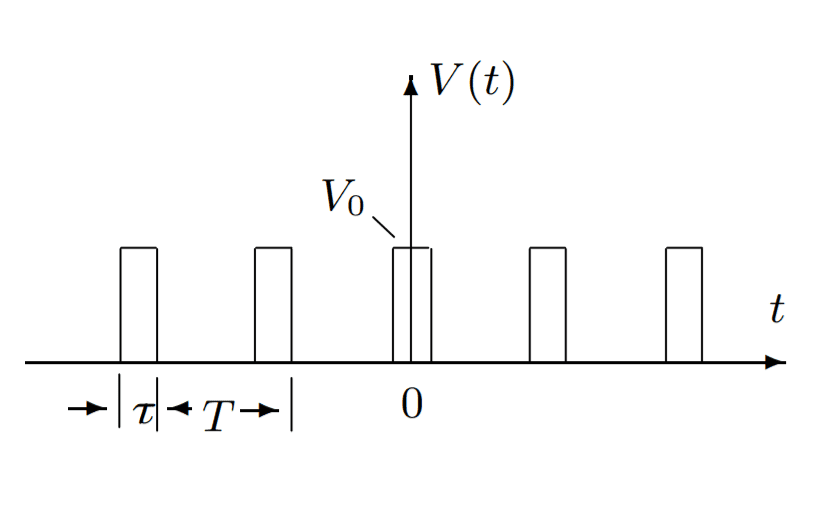
\includegraphics[width=0.9\linewidth]{image1.png}}
	\caption{Прямоугольные импульсы}
    \end{minipage}
    \begin{minipage}[h]{0.5\linewidth}
	\center{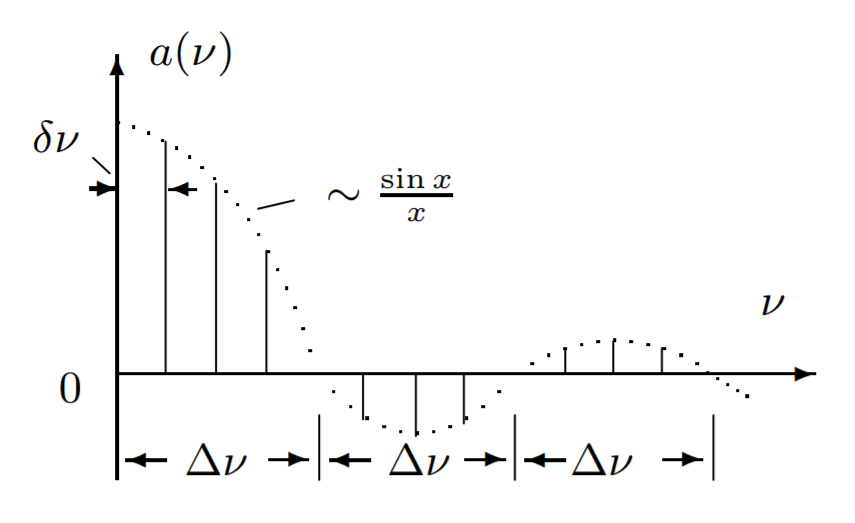
\includegraphics[width=0.9\linewidth]{image2.png}}
	\caption{Спектр последовательности прямоугольных импульсов}
    \end{minipage}
\end{figure}
	
Назовем \textit{шириной спектра} $\Delta \omega$ расстояние от главного максимума ($\omega =0$) до первого нуля огибающей, возникающего при $n=\dfrac{2\pi}{\tau \Omega_{1}}$. При этом 
	
\begin{equation}
	\Delta \omega \tau \backsimeq 2 \pi, \text{или }  \Delta \nu \Delta t \backsimeq 1
\label{eq5}
\end{equation}
		
Полученное соотношение взаимной связи интервалов $\Delta \nu$ и $\Delta t$ является частным случаем соотношения неопределенности в квантовой механике.
	
\item \textbf{Периодическая последовательность цугов} гармонического колебания $V_{0}\cos(\omega_{0}t)$ с длительностью цуга $\tau$ и периодом повторения $T$ (рис. 3).
	
Функция $f(t)$ снова является четной относительно $t=0$. Коэффициент при $n$-й гармонике равен

\begin{equation}
    a_{n}=\dfrac{2}{T}\int\limits_{-\frac{\tau}{2}}^{\frac{\tau}{2}}V_{0}\cos(\omega_{0}t)\cos(n \Omega_{1} t)dt=V_{0}\dfrac{\tau}{T} \bigg(\dfrac{\sin[(\omega_{0}-n\Omega_{1})\frac{\tau}{2}]}{(\omega_{0}-n\Omega_{1})\frac{\tau}{2}}+\dfrac{\sin[(\omega_{0}+n\Omega_{1})\frac{\tau}{2}]}{(\omega_{0}+n\Omega_{1})\frac{\tau}{2}} \bigg)
\label{eq6}
\end{equation}
	
Зависимость для случая, когда $\frac{T}{\tau}$ равно целому числу, представлена на рис. 4. Сравнивая спектр последовательности прямоугольных импульсов и цугов мы видим, что они аналогичны, но их максимумы сдвинуты по частоте на величину $\omega_{0}$.
	
\begin{figure}[h]
    \begin{minipage}[h]{0.5\linewidth}
	\center{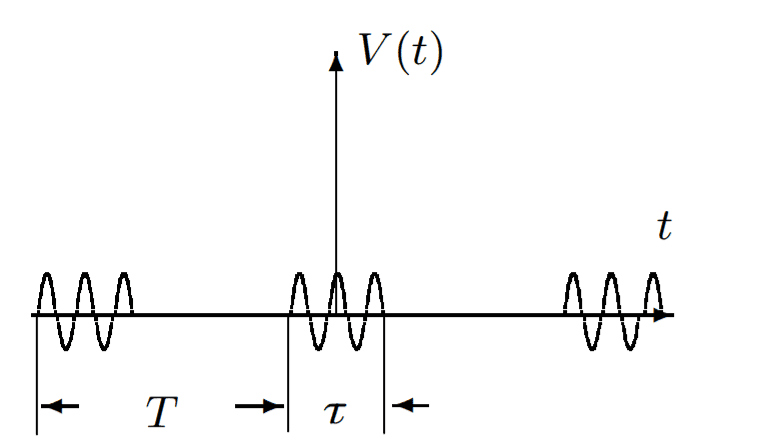
\includegraphics[width=0.9\linewidth]{image3.png}}
	\caption{Последовательность цугов}
    \end{minipage}
    \begin{minipage}[h]{0.5\linewidth}
	\center{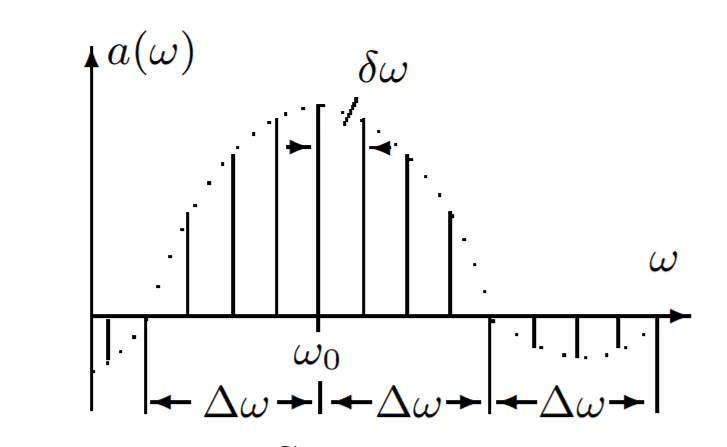
\includegraphics[width=0.9\linewidth]{image4.png}}
	\caption{Спектр последовательности цугов}
    \end{minipage}
\end{figure}

\item \textbf{Амплитудно-модулированные колебания.} Рассмотрим гармонические колебания высокой частоты $\omega_{0}$ , амплитуда которых медленно меняется по гармоническому закону с частотой $\Omega$ ($\Omega \ll \omega_{0})$) (рис. 5):

\begin{equation}
    f(t)=A_{0}[1+m\cos\Omega t]\cos \omega_{0}t
\label{eq7}
\end{equation}	

Коэффициент $m$ называют \textbf{глубиной модуляции}. При $m<1$ амплитуда колебаний меняется от минимальной $A_{min}=A_{0}(1-m)$ до максимальной $A_{max}=A_{0}(1+m).$ Глубина модуляции может быть представлена в виде
	
\begin{equation}
	 m=\dfrac{A_{max}-A_{min}}{A_{max}+A_{min}}
\label{eq8}
\end{equation}
	
Простым тригонометрическим преобразованием можно найти спектр амплитудно - модулированных колебаний:

\begin{equation}\label{a}
	f(t)=A_{0}\cos(\omega_{0} t)+\dfrac{A_{0}m}{2}\cos(\omega_{0}+\Omega)t+\dfrac{A_{0}m}{2}\cos(\omega_{0}-\Omega)t.
\end{equation}
		
\begin{figure}[h]
    \begin{minipage}[h]{0.5\linewidth}
	\center{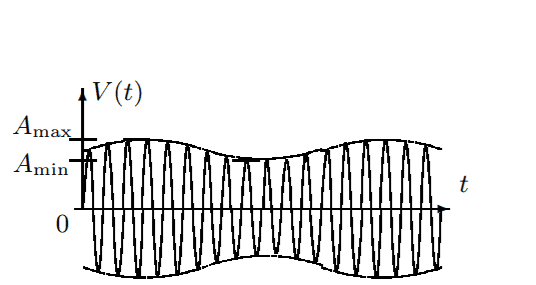
\includegraphics[width=0.9\linewidth]{image5.png}}
	\caption{Модулированные гармонические колебания}
    \end{minipage}
    \begin{minipage}[h]{0.5\linewidth}
	\center{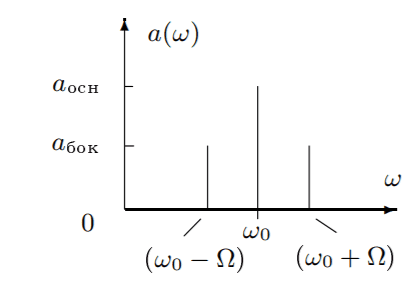
\includegraphics[width=0.9\linewidth]{image6.png}}
	\caption{Спектр модулированных гармонических колебаний}
    \end{minipage}
\end{figure}
		
Спектр таких колебаний содержит три составляющих  основную компоненту и две боковых (рис. 6). Первое слагаемое в правой части представляет собой исходное немодулированное колебание с основной (несущей) частотой $\omega_{0}$ и амплитудой $a_{осн} = A_{0}$ . Второе и третье слагаемые соответствуют новым гармоническим колебаниям с частотами $\omega_{0} + \Omega$ и $\omega_{0} - \Omega$. Амплитуды этих двух колебаний одинаковы и составляют $\dfrac{m}{2}$ от амплитуды немодулированного колебания: $a_{бок} = \dfrac{A_{0}m}{2}$. Начальные фазы всех трех колебаний одинаковы.

\end{enumerate}

\section{Экспериментальная установка.}
В работе изучаются спектры периодических электрических сигналов 
различной формы (последовательности прямоугольных импульсов и цугов, 
а также амплитудно- и фазо-модулированных гармонических колебаний). 
Спектры этих сигналов наблюдаются с помощью спектроанализатора, входящего в состав USB-осциллографа и сравниваются с рассчитанными теоретически. Схема установки изображена на рис.\ref{ustanovka}

\begin{figure}[h]
    \centering
    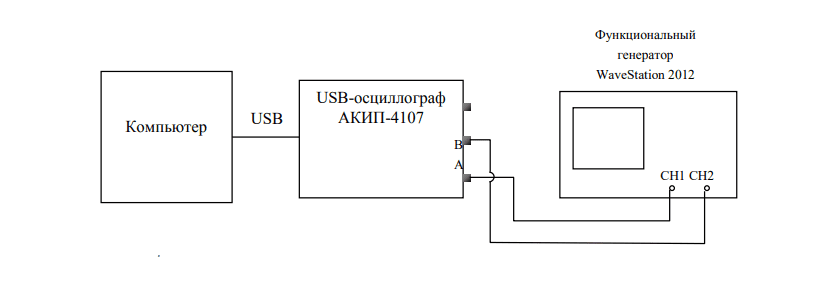
\includegraphics[width=17cm]{image7.png}
    \caption{Схема экспериментальной установки}
    \label{ustanovka}
\end{figure}

Функциональный генератор $WaveStation 2012$ позволяет сформировать два 
различных электрических сигнала, которые выводятся на два независимых канала – "CH1" и "CH2". Сигнал с канала "CH1" подается на вход "А", а сигнал с канала "CH2" – на вход "В" USB-осциллографа. Затем эти сигналы подаются на вход компьютера через USB-соединение. При работе USB-осциллографа в режиме осциллографа, на экране компьютера можно наблюдать каждый из сигналов в отдельности, а также их произведение. В режиме спектроанализатора можно наблюдать спектры этих сигналов.
При включении функционального генератора, на его экране отображается информация о параметрах электрического сигнала.

\section{Экспериментальная часть}

\begin{enumerate}
    \item Ознакомились с устройством приборов: генератора сигналов произвольний формы, компьтерной программы, используемой для отображения сигнала с осциллографа.
    \item Подключили один из выходов генеротора к одному из каналов осциллографа, подключили приборы в сеть.
\end{enumerate}

\subsection{Исследование спектра периодической последовательности прямоугольных импульсов и проверка соотношений неопределённостей}

\begin{enumerate}
    \item Настроили генерацию прямоугольных импульсов со следующими параметрами: частота повторения $\nu_{\text{повт}} = 1 \text{кГц}$, Длительность импульса $\tau = \frac{T}{20} = \frac{1}{20\nu_{\text{повт}}} = 50 \text{мкс}$.
    \item Получили устойчивую картину колебаний (рис. \ref{f1}) и спектр (преобразование Фурье) сигнала (рис. \ref{f2}).

    \begin{figure}[h]
        \begin{minipage}[h]{0.5\linewidth}
    	\center{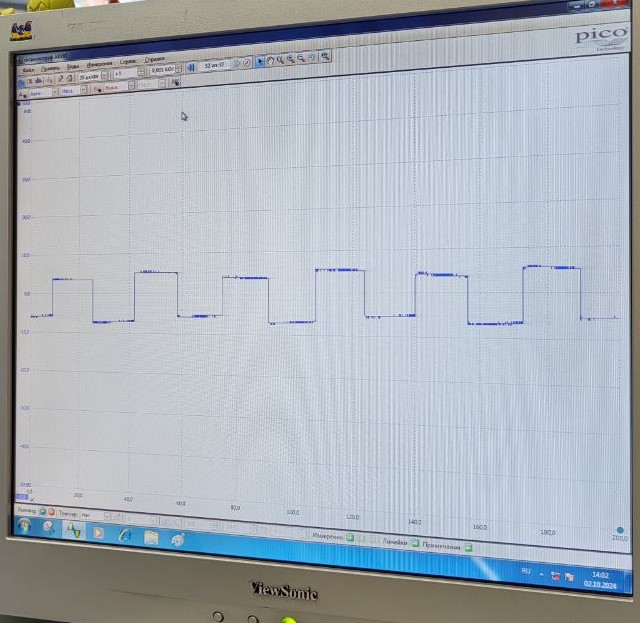
\includegraphics[width=0.6\linewidth]{f1.jpg}}
    	\caption{Устойчивая картина колебаний прямоугольных импульсов}
            \label{f1}
        \end{minipage}
        \begin{minipage}[h]{0.5\linewidth}
    	\center{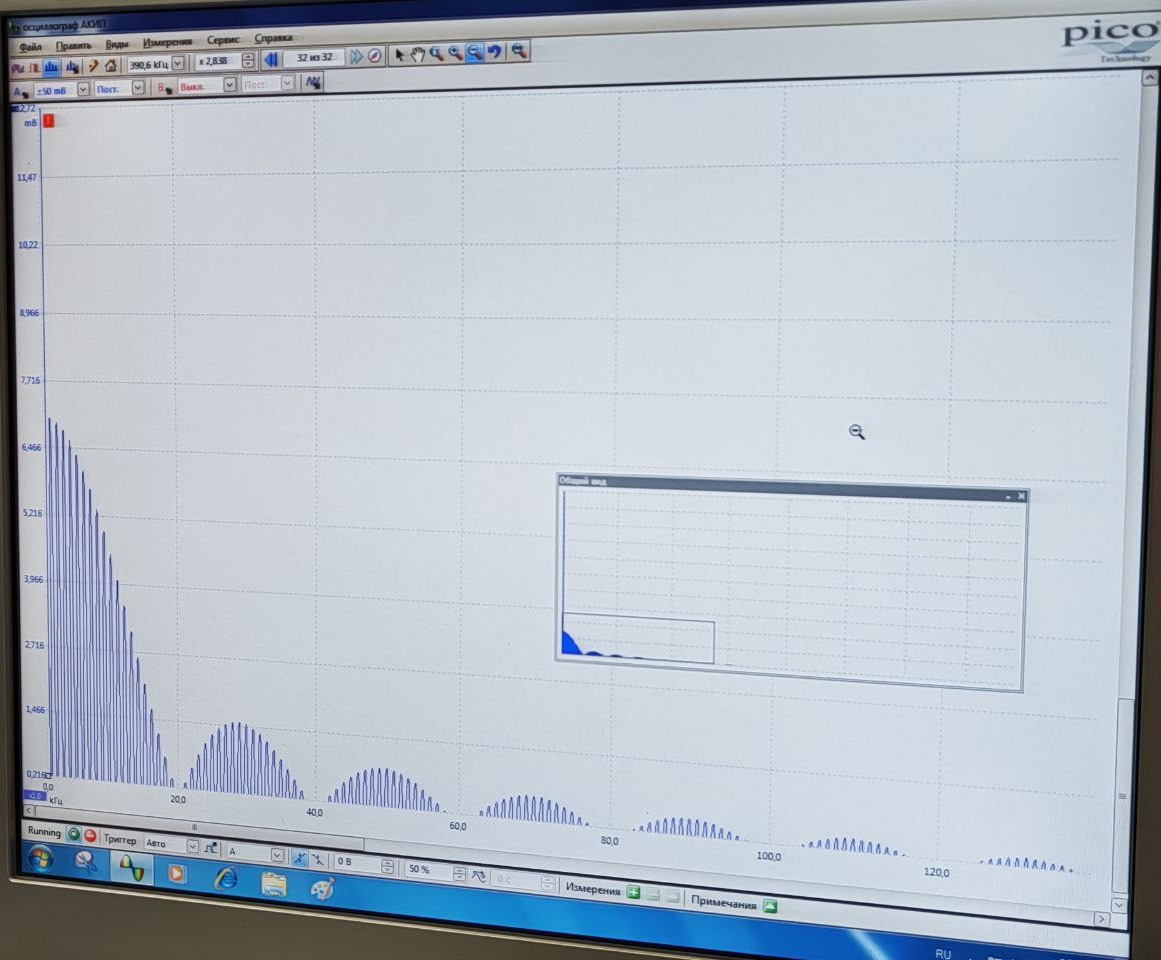
\includegraphics[width=0.7\linewidth]{f2.jpg}}
    	\caption{Спектр последовательности прямоуольных импульсов}
            \label{f2}
        \end{minipage}
        \begin{minipage}[h]{0.5\linewidth}
    	\center{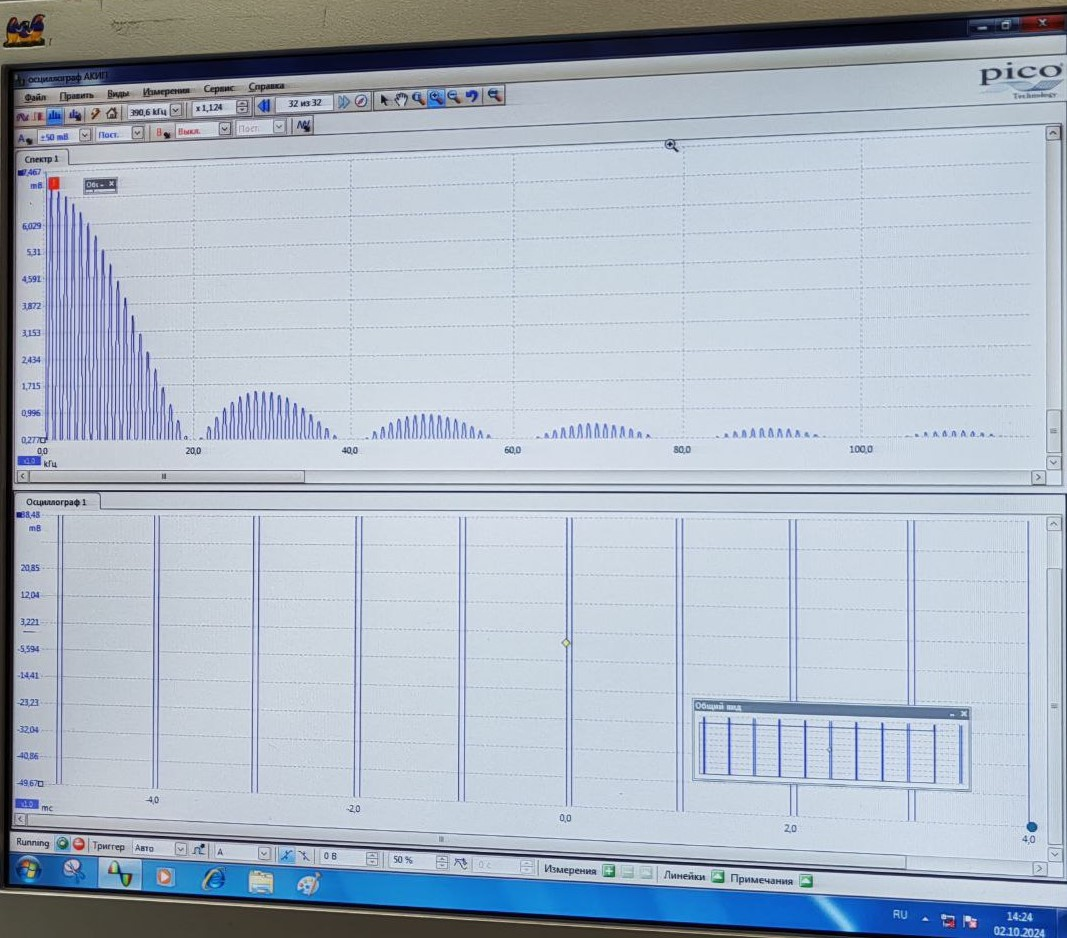
\includegraphics[width=0.6\linewidth]{f3.jpg}}
    	\caption{Сигнал и спектр}
            \label{f3}
        \end{minipage}
    \end{figure}

    \item Будем изменять параметры сигнала, наблюдаем за изменением спектра:
    \begin{enumerate}
        \item изменяем $\nu_{\text{повт}}$ при фиксированном $\tau$: изменяется количество импульсов.

        \begin{figure}[h]
            \begin{minipage}[h]{0.5\linewidth}
        	\center{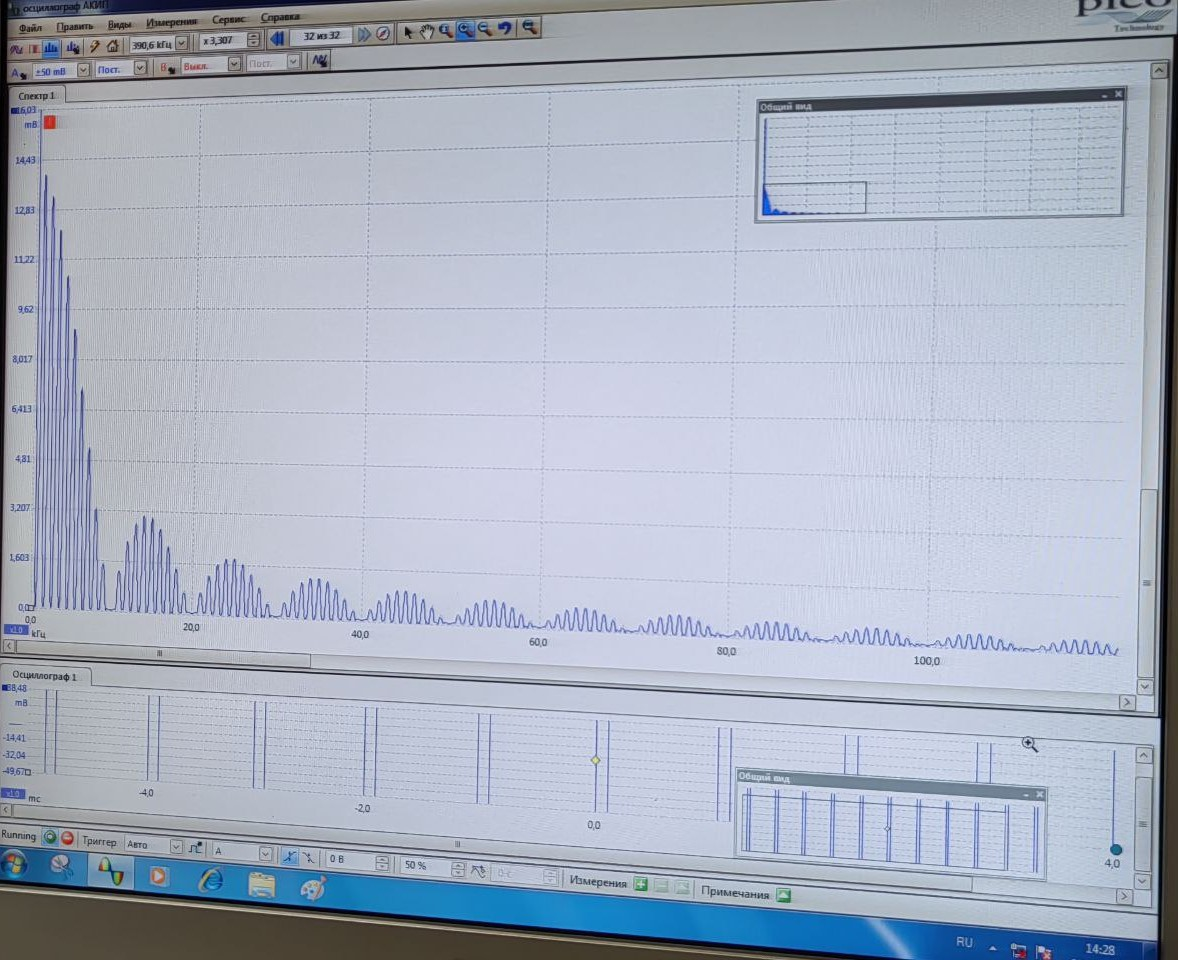
\includegraphics[width=0.7\linewidth]{f8.jpg}}
        	\caption{$\nu_{\text{повт}} = 500 \text{Гц}, \tau = 50 \text{мкс}$.}
            \end{minipage}
            \begin{minipage}[h]{0.5\linewidth}
        	\center{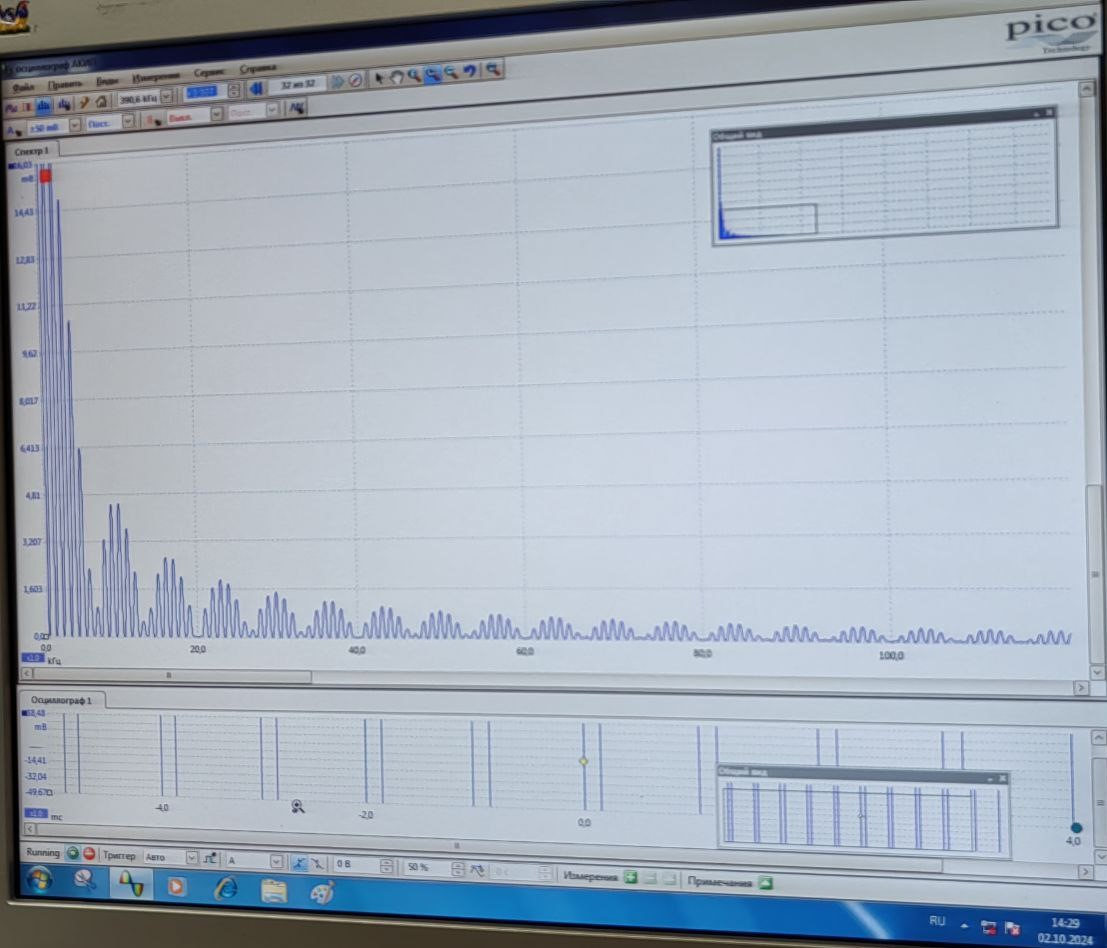
\includegraphics[width=0.7\linewidth]{f9.jpg}}
        	\caption{$\nu_{\text{повт}} = 1500 \text{Гц}, \tau = 50 \text{мкс}$.}
            \end{minipage}
            \begin{minipage}[h]{0.5\linewidth}
        	\center{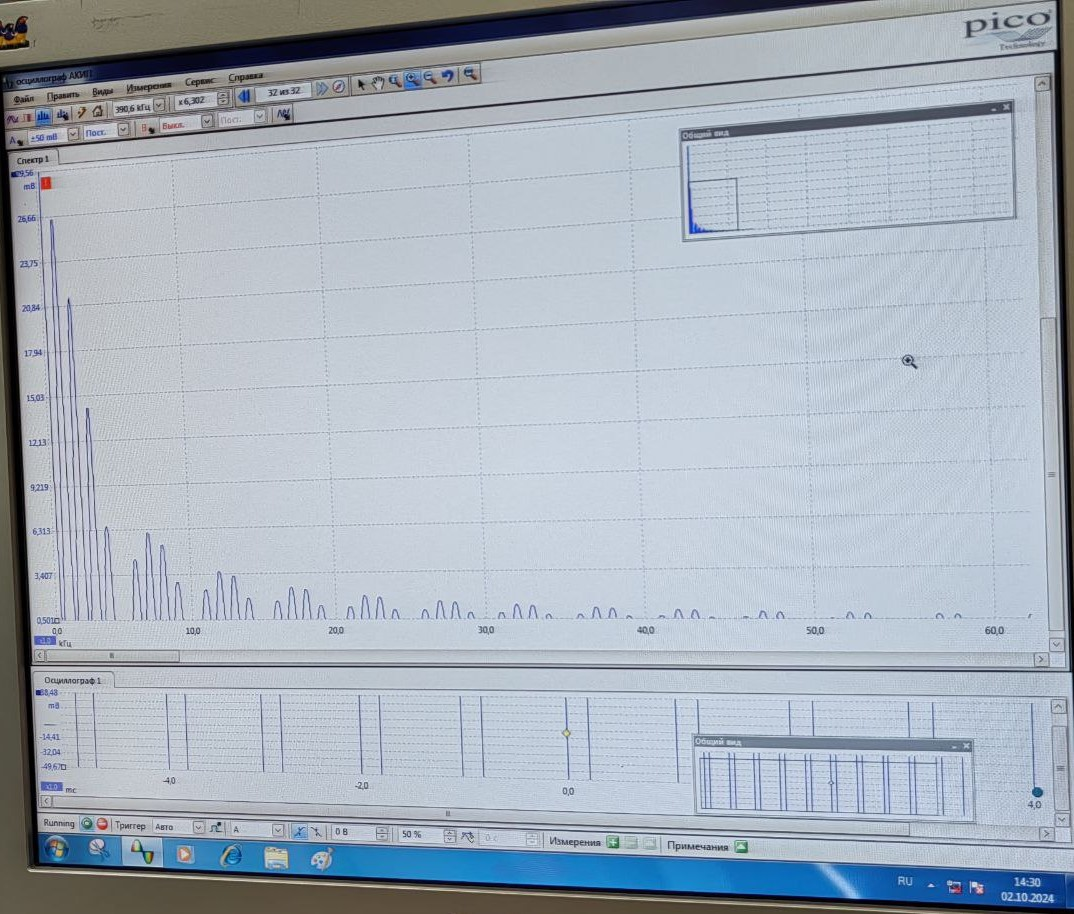
\includegraphics[width=0.7\linewidth]{f10.jpg}}
        	\caption{$\nu_{\text{повт}} = 2000 \text{Гц}, \tau = 50 \text{мкс}$.}
            \end{minipage}
            \begin{minipage}[h]{0.5\linewidth}
        	\center{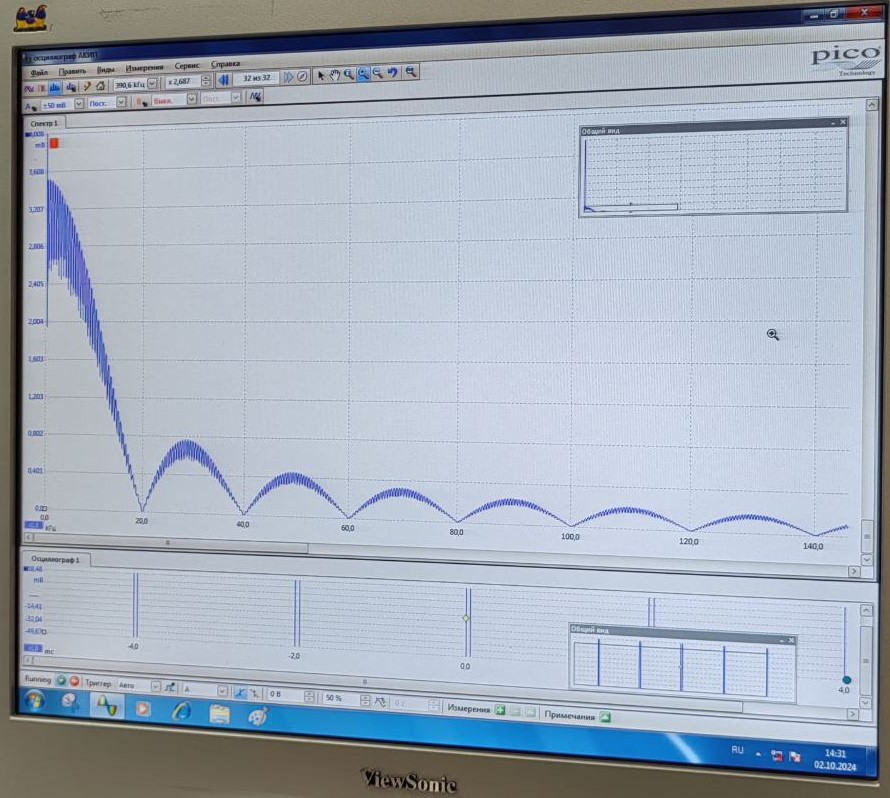
\includegraphics[width=0.7\linewidth]{f4.jpg}}
        	\caption{$\nu_{\text{повт}} = 1000 \text{Гц}, \tau = 50 \text{мкс}$.}
            \end{minipage}
            \begin{minipage}[h]{0.5\linewidth}
        	\center{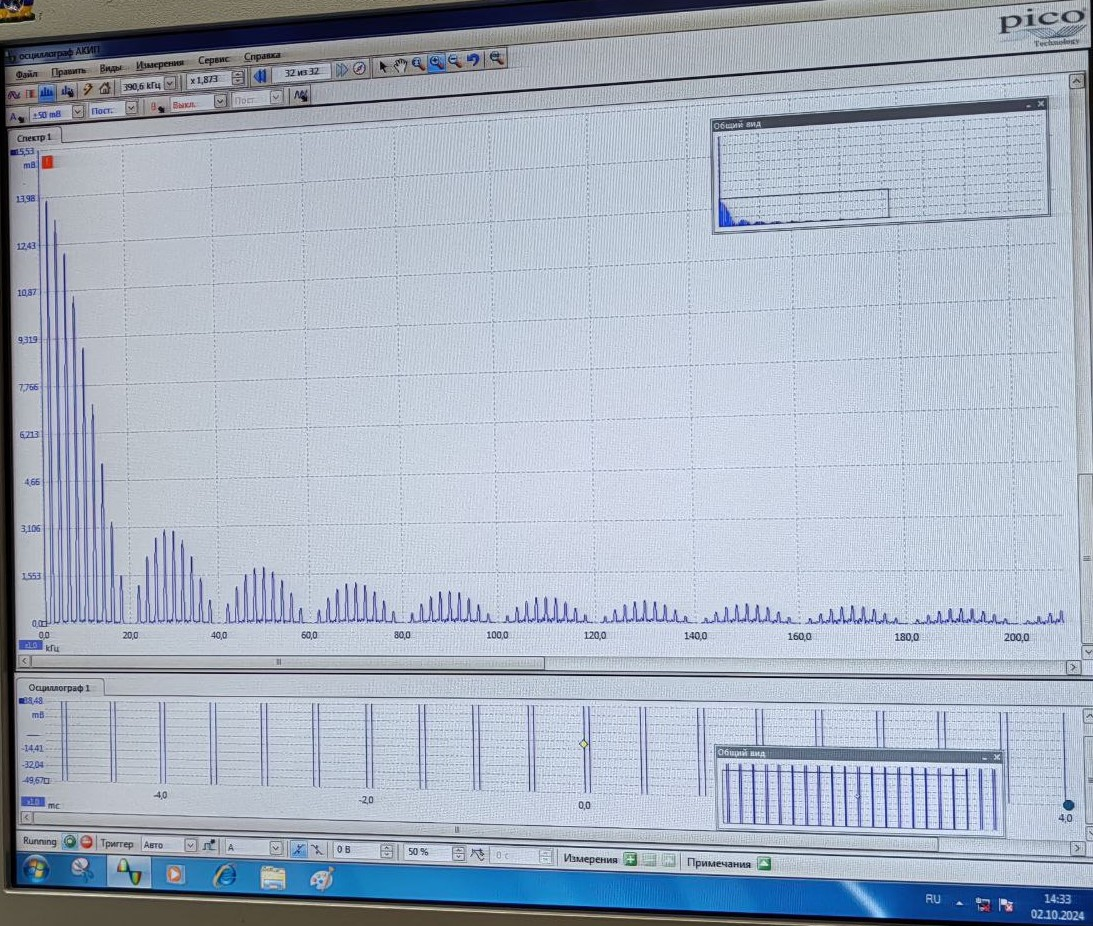
\includegraphics[width=0.7\linewidth]{f6.jpg}}
        	\caption{$\nu_{\text{повт}} = 1000 \text{Гц}, \tau = 150 \text{мкс}$.}
            \end{minipage}
            \begin{minipage}[h]{0.5\linewidth}
        	\center{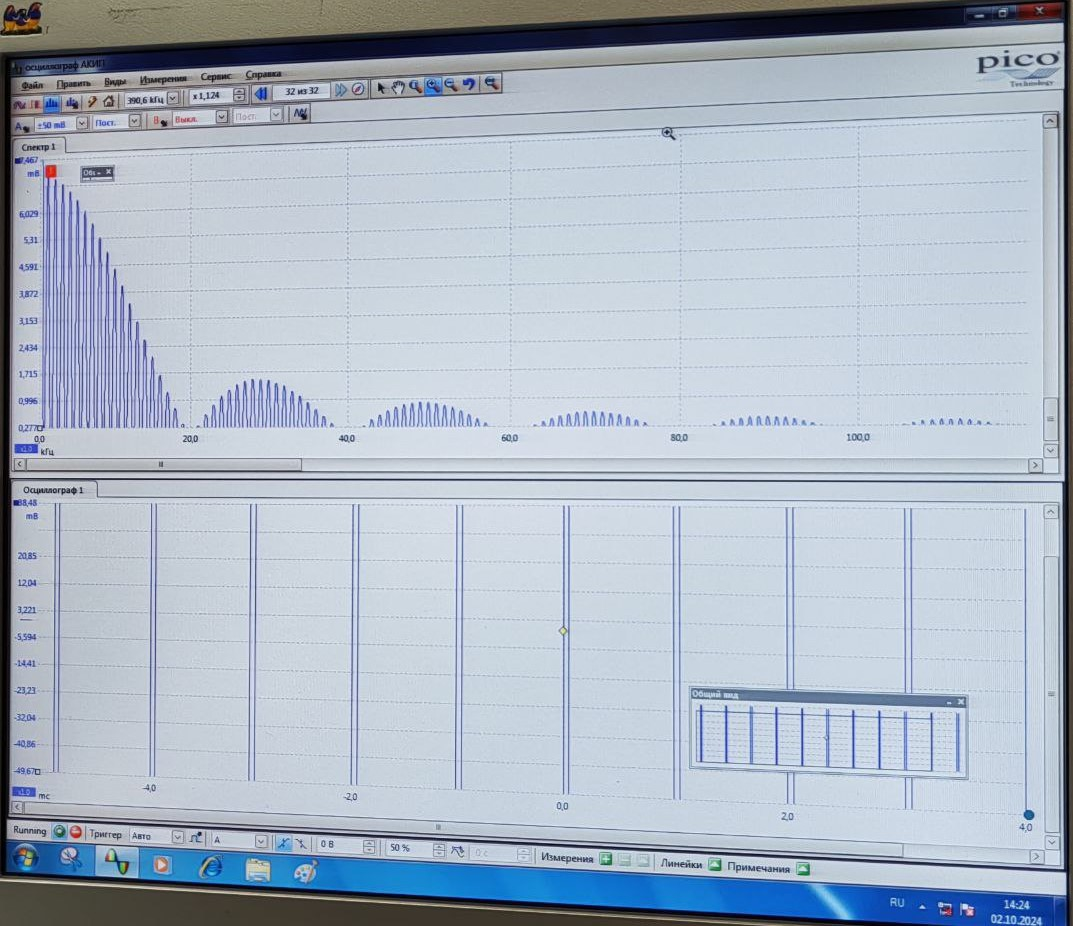
\includegraphics[width=0.7\linewidth]{f7.jpg}}
        	\caption{$\nu_{\text{повт}} = 1000 \text{Гц}, \tau = 200 \text{мкс}$.}
            \end{minipage}
        \end{figure}

        \item изменяем $\tau$ при фиксированном $\nu_{\text{повт}}$: изменяется длительность импульсов.
            
        \end{enumerate}

    \item Принекоторых фиксированных параметрах ($\nu_{\text{повт}} = 1 \text{кГц}$, $\tau = 50 \text{мкс}$) измерим амплитуды $a_n$ и частоты $\nu_n$ нескльких спектральных компонент (гармоник). Результаты занесём в таблицу \ref{tab1}.

    \begin{figure}[h]
        \center{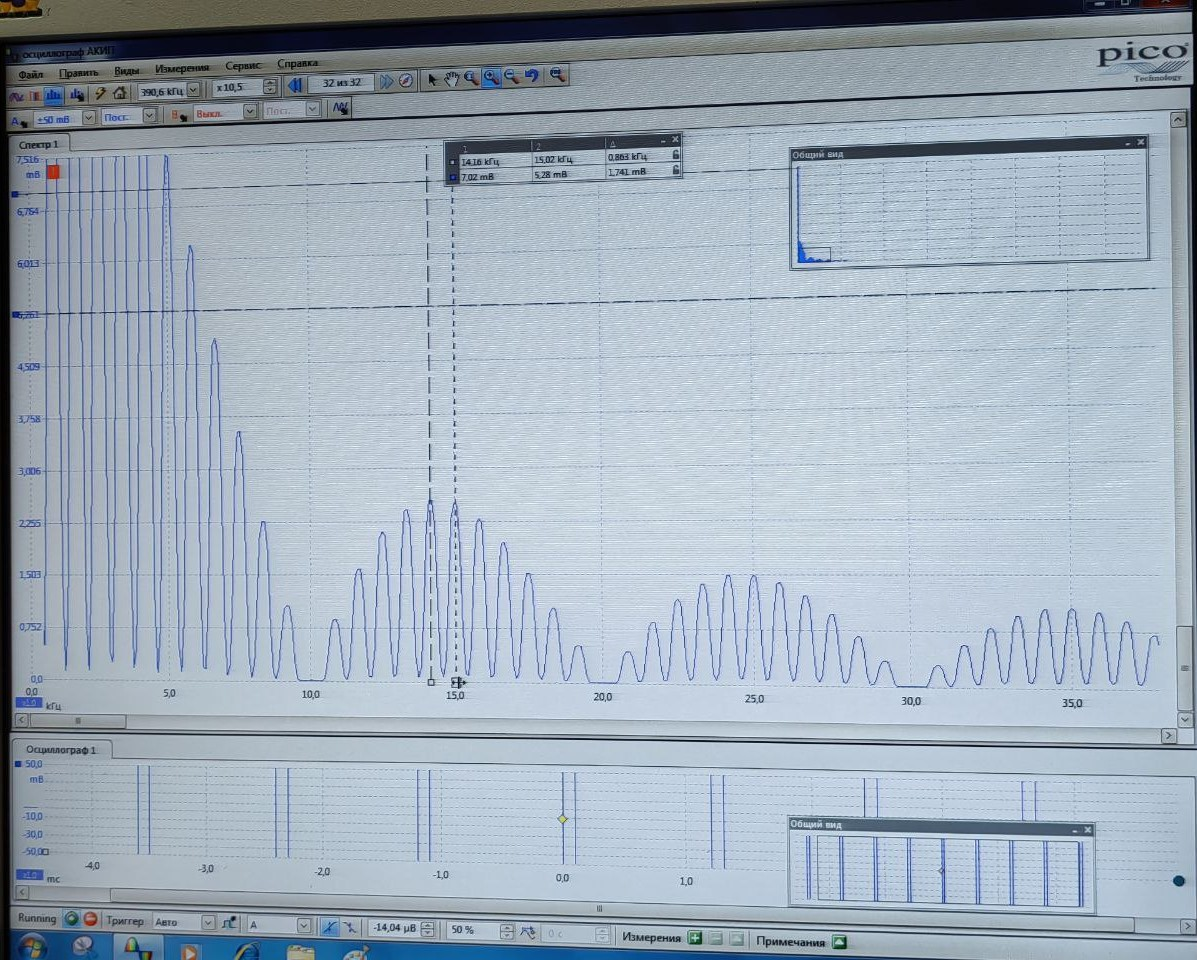
\includegraphics[width=0.6\linewidth]{f11.jpg}}
        \caption{Устойчивая картина колебаний прямоугольных импульсов}
        \label{f11}
    \end{figure}

    \[ \nu_n = \frac{n}{T}, \text{ } |a_n| = \frac{|\sin{\frac{\pi n \tau}{T}}|}{\pi n} = \frac{\tau}{T}\frac{|\sin{\pi \nu_n \tau}|}{\pi \nu_n \tau} \].

    \begin{table}[h]
	\centering
		\begin{tabular}{|c|c|c|c|c|c|c|c|c|}
			\hline
                n & 1 & 2 & 3 & 4 & 5 & 6 & 7 & 8 \\ \hline
                $\nu_n^{\text{эксп}}, \text{Гц}$ & 1002 & 1980 & 2995 & 4009 & 5023 & 6001 & 7015 & 7993 \\ \hline
                $\nu_n^{\text{теор}}, \text{Гц}$ & $10^3$ & $2 \cdot 10^3$ & $3 \cdot 10^3$ & $4 \cdot 10^3$ & $5 \cdot 10^3$ & $6 \cdot 10^3$ & $7 \cdot 10^3$ & $8 \cdot 10^3$ \\ \hline
                $|a_n|^{\text{эксп}}$, \text{мВ} & 7.025 & 6.93 & 6.79 & 6.6 & 6.353 & 6.061 & 5.707 & 5.34 \\ \hline
                $|a_n/a_1|^{\text{эксп}}$ & 1 & 0.986 & 0.967 & 0.939 & 0.904 & 0.863 & 0.812 & 0.760 \\ \hline
                $|a_n/a_1|^{\text{теор}}$ & 1 & 0.984 & 0.963 & 0.935 & 0.900 & 0.858 & 0.810 & 0.757 \\ \hline
		\end{tabular}
	\caption{Результаты измерений и вычислений}
        \label{tab1}
    \end{table}

    \begin{table}[h]
	\centering
		\begin{tabular}{|c|c|}
			\hline
                $\tau, \text{мкс}$ &  $\Delta \nu, \text{кГц}$ \\ \hline
                20 & 50.09 \\ \hline
                40 & 25.01 \\ \hline
                60 & 16.99 \\ \hline
                80 & 12.5 \\ \hline
                100 & 10.0 \\ \hline
		\end{tabular}
            \hspace{.02\textwidth}
            \begin{tabular}{|c|c|}
			\hline
                $\tau, \text{мкс}$ &  $\Delta \nu, \text{кГц}$ \\ \hline
                120 & 8.447 \\ \hline
                140 & 6.99 \\ \hline
                160 & 5.995 \\ \hline
                180 & 5.497 \\ \hline
                200 & 5.0 \\ \hline
		\end{tabular}
	\caption{Зависимость ширины спектра сигнала от длительности импульса}
        \label{tab2}
    \end{table}
    \begin{table}[h]
	\centering
		\begin{tabular}{|c|c|}
			\hline
                $T, \text{мкс}$ &  $\delta \nu, \text{кГц}$ \\ \hline
                200 & 5.01 \\ \hline
                700 & 1.453 \\ \hline
                1200 & 0.832 \\ \hline
                1700 & 0.584 \\ \hline
		\end{tabular}
            \hspace{.02\textwidth}
            \begin{tabular}{|c|c|}
			\hline
                $T, \text{мкс}$ &  $\delta \nu, \text{кГц}$ \\ \hline
                2200 & 0.429 \\ \hline
                2700 & 0.361 \\ \hline
                3200 & 0.3 \\ \hline
                3700 & 0.28 \\ \hline
		\end{tabular}
	\caption{Зависимость разности частот между соседними гармониками от периода повторений}
        \label{tab3}
    \end{table}

     \item Зафиксируем период повторений $Т = 1 \text{мс}$ прямоугольного сигнала. Изменяя длительность импульса $\tau$ в диапазоне от $\tau = \frac{T}{50}$ до $\tau = \frac{T}{5}$, измерим полную ширину спектра сигнала $\Delta \nu$ -- от центра спектра до гармоники с нулевой амплитудой (таблица \ref{tab2}).

    \item Зафиксируем длительность импульса прямоугольного сигнала $\tau = 100 \text{мкс}$. Изменяя период повторения $T$ в диапазоне от $2\tau$ до $50\tau$, измерим расстояние $\delta \nu = \nu_{n+1} - \nu_{n}$ между соседними гармониками спектра (таблица \ref{tab3}).

    \item Построим графики зависимостей $\Delta \nu(1/\tau)$ (рис. \ref{graf1}) и $\delta \nu(1/T)$ (рис. \ref{graf2}).Проведём наилучшие прямые и определим их наклон. 

    \[ k_1 = 1.00035, \text{ } k_2 = 1.0042. \]
    
    Так же убедимся в справедливости соотношений неопреденности:

    \[ \tau \cdot \Delta \nu \approx 1 \Longleftrightarrow \tau \cdot \Delta \omega \approx 2\pi\]
    \[ T \cdot \delta \nu \approx 1 \Longleftrightarrow T \cdot \delta \omega \approx 2\pi\]

    Чем больше длительность сигнала $\tau$ (либо больше интервал времени $T$, в течении которого происходит его заметное изменение), тем уже спектр сигнала $\Delta \omega$, и, наоборот, чем короче сигналы (или быстрее происходит изменение сигнала), тем шире его спектр, т.е. требуется более длинный сигнал, образующих в сумме данный сигнал. \textit{Соотношения неопределённостей} выполняются.
\end{enumerate}

\subsection{Наблюдения спектра периодической последовательности цугов}

\begin{enumerate}
    \item Истановим генератор на режим подачи периодических импульсов синусоидальной формы (цугов) со следующими параметрами: несущая частота $ \nu_0 = 50 \text{Гц} $, период повторения $ T = 1 мс $, число периодов синусоиды в одном импульсе $ N = 5 $ (что соответствует длительности импульса $\tau = N/\nu_0 = 100 мкс $). Получили на экране осциллографа устойчивую картину согнала.

    \begin{figure}[h]
        \center{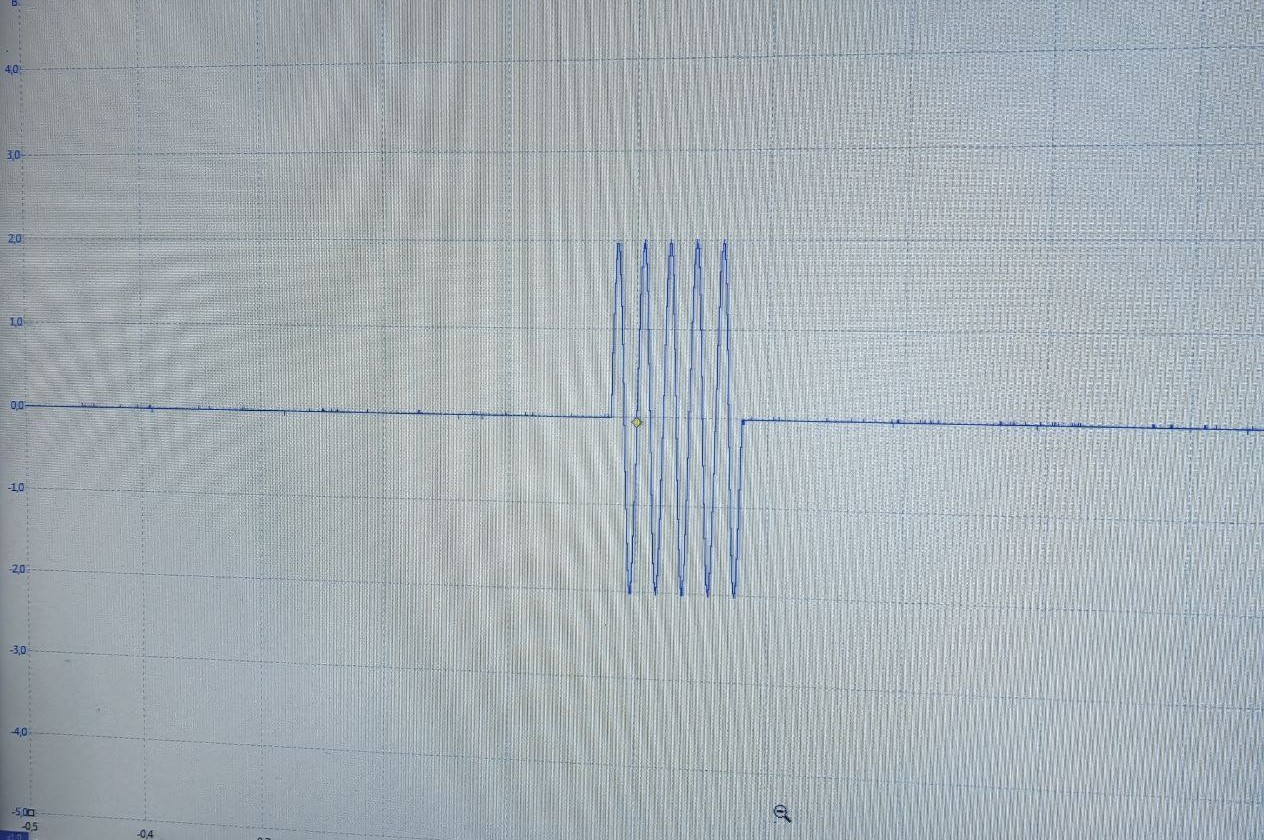
\includegraphics[width=0.7\linewidth]{f12.jpg}}
        \caption{Устойчивая картина цуга}
        \label{f12}
    \end{figure}

    \item Получим на экране осциллографа спектр сигнала. Изменяя параметры сигнала $\nu_0$, $T$ и $N$ наблюдаем, как изменяется вид спектра.

    \begin{figure}[h]
        \begin{minipage}[h]{0.5\linewidth}
            \center{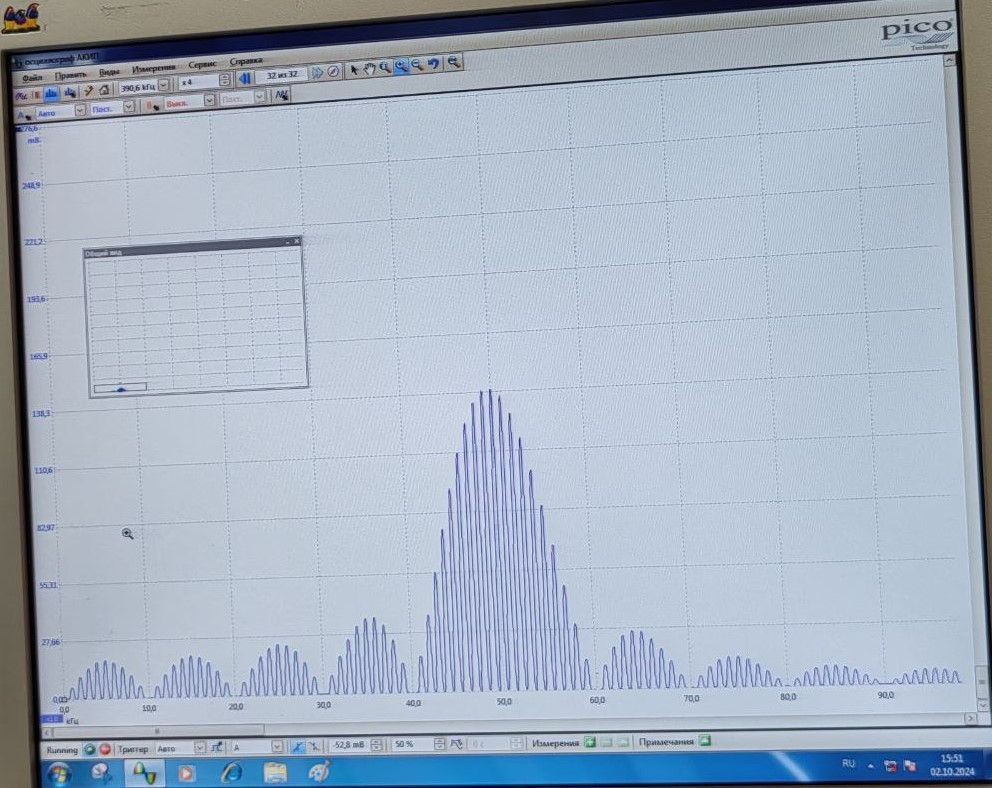
\includegraphics[width=0.85\linewidth]{f13.jpg}}
            \caption{$\nu_0 = 50 \text{Гц}, T = 1 \text{мс}$, N = 5.}
        \end{minipage}
        \begin{minipage}[h]{0.5\linewidth}
            \center{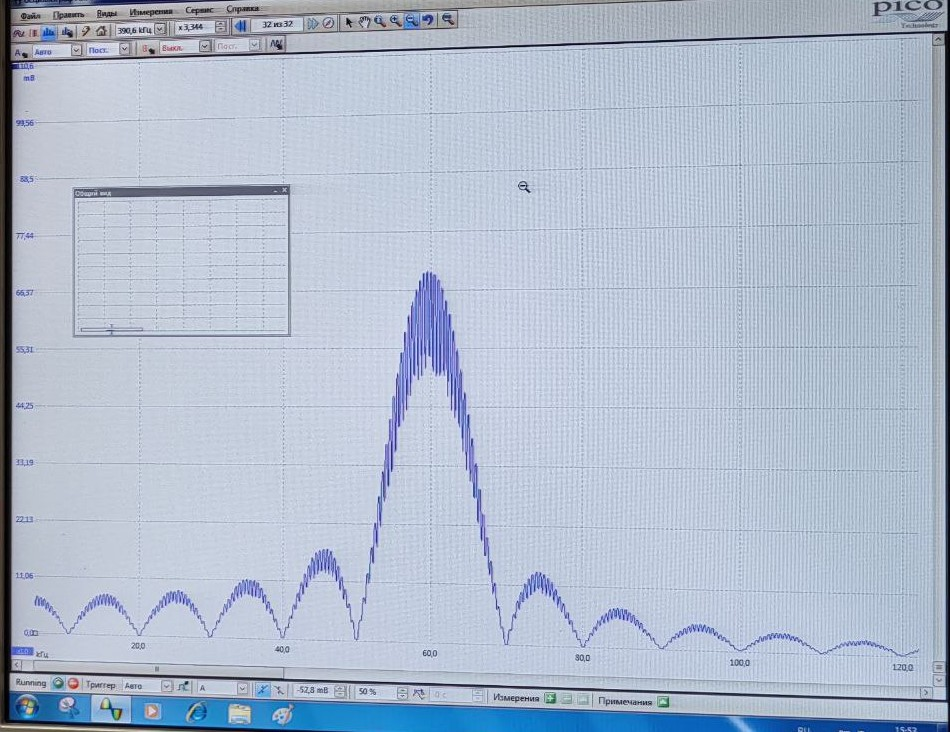
\includegraphics[width=0.85\linewidth]{f14.jpg}}
            \caption{$\nu_0 = 60 \text{Гц}, T = 2 \text{мс}$, N = 6.}
        \end{minipage}
        \begin{minipage}[h]{0.5\linewidth}
            \center{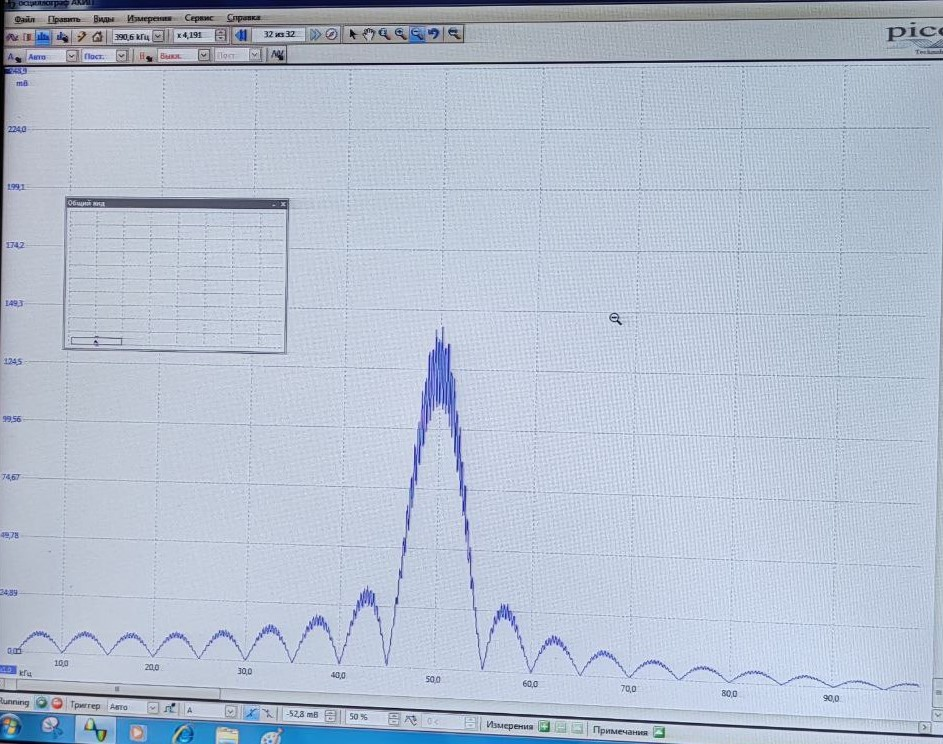
\includegraphics[width=0.85\linewidth]{f15.jpg}}
            \caption{$\nu_0 = 50 \text{Гц}, T = 3 \text{мс}$, N = 10.}
        \end{minipage}
    \end{figure}

    При изменении несущей частоты $\nu_0$ изменяется положение центр картины. При изменении симла периодов $N$ изменяется число дуг. При изменении периода повторений $T$ изменяется расстояние между импульсами.

    \item При параметрах сигнала, соответствующих сохранённых в предыдущем пункте изображениям, измерим положение центра спектра, его ширину $\Delta \nu$ и расстояние между гармониками $\delta \nu$. Результаты занесём в таблицу \ref{tab4}.

    \begin{table}[h]
	\centering
		\begin{tabular}{|c|c|c|c|c|c|c|}
			\hline
                  & $\nu_0, \text{Гц}$ & $T$, \text{мс} & $N$ & $\nu^{\text{центр}}, \text{Гц}$ & $\Delta \nu, \text{кГц}$ &$\delta \nu, \text{кГц}$ \\ \hline
                1 & 50 & 1 & 5 & 50 & 10 & 1.054 \\ \hline
                2 & 60 & 2 & 6 & 60 & 10 & 0.494 \\ \hline
                3 & 50 & 3 & 10 & 50 & 5 & 0.325 \\ \hline
		\end{tabular}
	\caption{Результаты измерений}
        \label{tab4}
    \end{table}

    \textbf{Теорема смещения: } смещение сигнала во времени на $\tau$ (запаздывание) приводит к умножению его спектра на $e^{-i\omega\tau}$.

    Теорема смещения и соотношения неопределённостей выполняются.
    
\end{enumerate}

\subsection{Исследование спектра амплитудно-модулированного сигнала}

\begin{enumerate}
    \item Установим на генераторе режим \textit{модулированного по амплитуде} синусоидального сигнала со следующими параметрами: несущая частота $\nu_0 = 50 \text{кГц}$, частота модуляции $\nu_{\text{мод}} = 2 \text{кГц}$, глубина модуляции $m = 0.5 (50 \%)$. Получим на экране осциллографа устойчивую картину сигнала (рис. \ref{f16}).

    \begin{figure}[h]
        \center{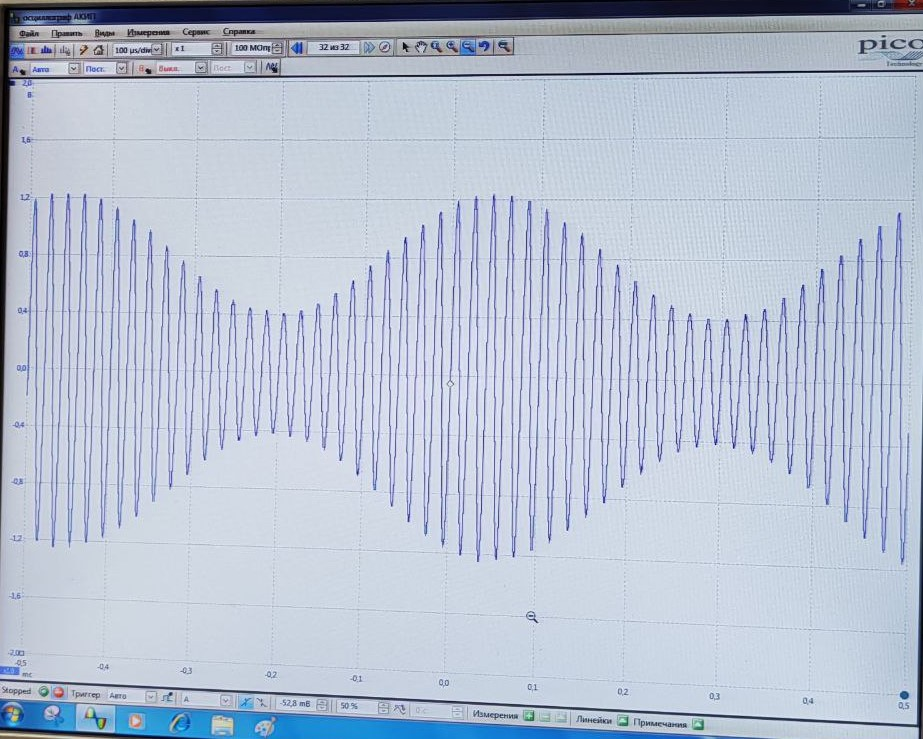
\includegraphics[width=0.7\linewidth]{f16.jpg}}
        \caption{Устойчивая картина амплитудно-модулированного сигнала}
        \label{f16}
    \end{figure}

    \item С помощью осциллографа (в режиме курсорных измерений) измерим максимальную $A_{max}$ и минимальную $A_{min}$ амплитуды сигнала.

    \[ A_{max} = 1.232 B, \text{ } A_{min} = 0.406 B, \text{ } m = \frac{A_{max} - A_{min}}{A_{max} + A_{min}} = \frac{1.232 - 0.406}{1.232 + 0.406} = 0.504 \rightarrow \textit{верно.} \]

    \item Получим на экране спектр сигнала. Измерим частоты центральной и боковой гармоник (в режиме курсорных измерений). Изменяя несущую частоту $\nu_0$ и частоту модуляции $\nu_{\text{мод}}$, наблюдаем, как изменяется положение спектральных линий.

    При изменении частоты модуляции изменяется положение боковых амплитуд. При изменении несущей частоты изменяется положение основной амплитуды.

    \begin{figure}[h]
        \begin{minipage}[h]{0.5\linewidth}
            \center{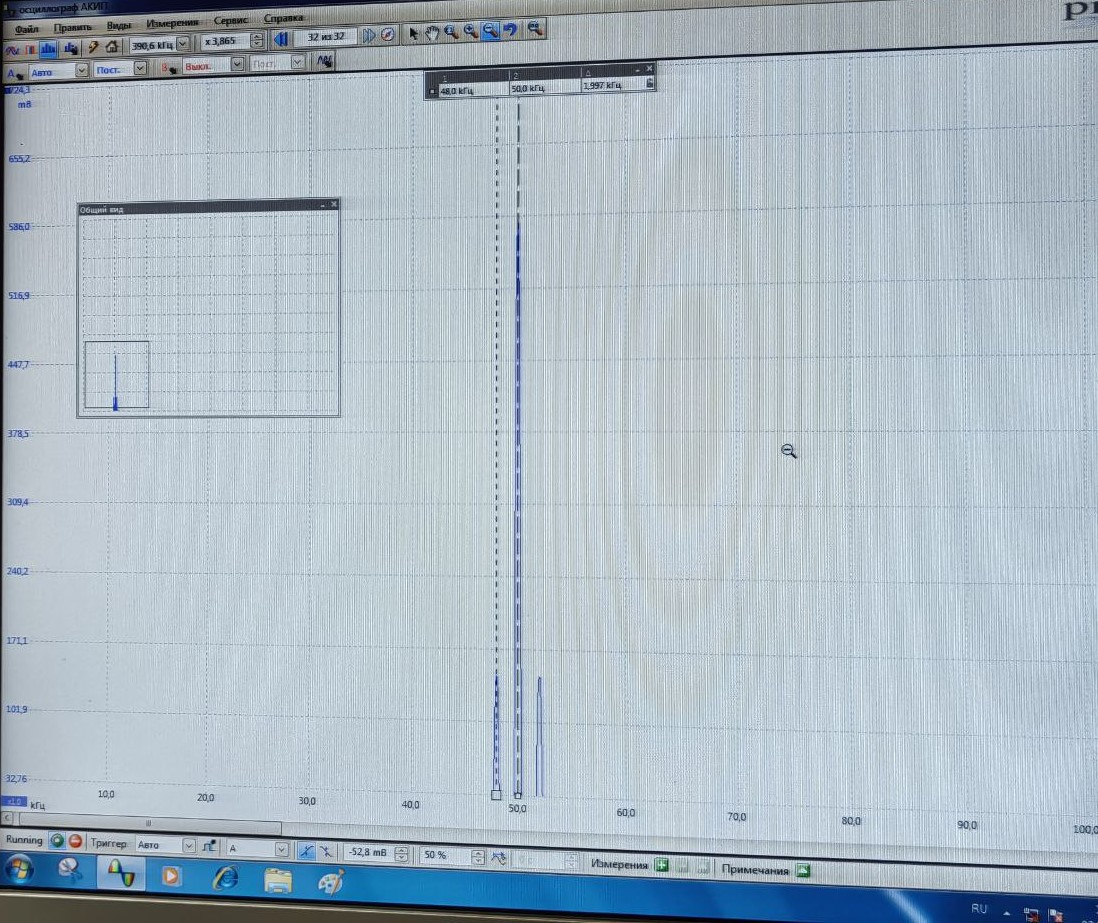
\includegraphics[width=0.8\linewidth]{f17.jpg}}
            \caption{$\nu_0 = 25 \text{Гц}$, $\nu = 1 \text{кГц}$.}
        \end{minipage}
        \begin{minipage}[h]{0.5\linewidth}
            \center{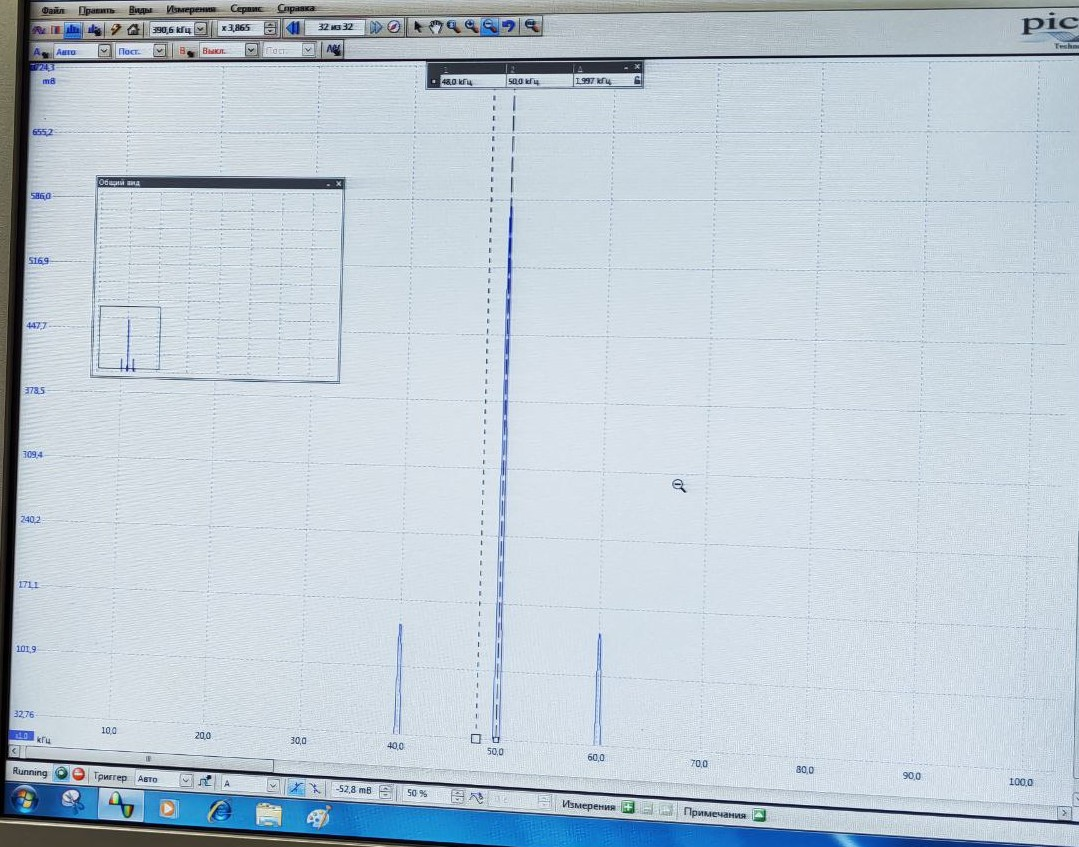
\includegraphics[width=0.8\linewidth]{f18.jpg}}
            \caption{$\nu_0 = 25 \text{Гц}$, $\nu = 1.5 \text{кГц}$.}
        \end{minipage}
        \begin{minipage}[h]{0.5\linewidth}
            \center{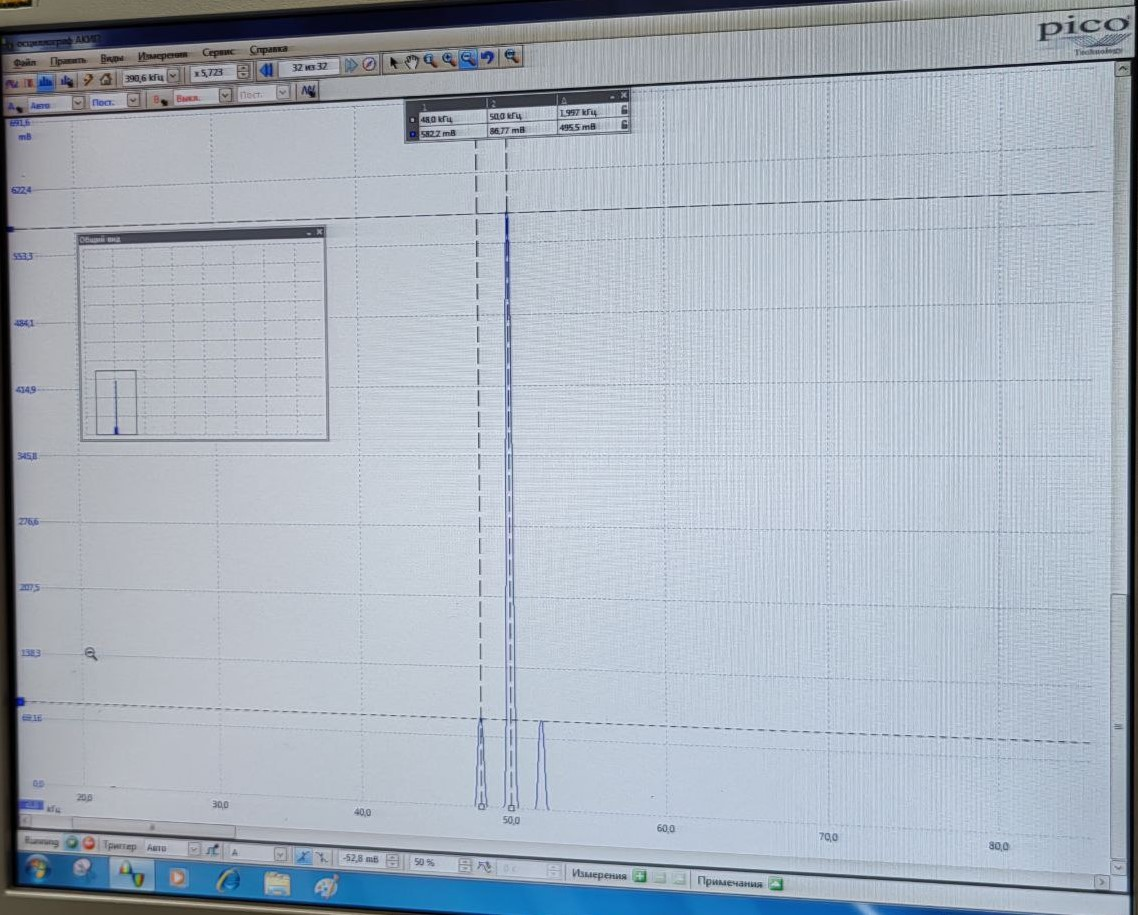
\includegraphics[width=0.8\linewidth]{f19.jpg}}
            \caption{$\nu_0 = 25 \text{Гц}$, $\nu = 500 \text{кГц}$.}
        \end{minipage}
    \end{figure}

    \item Изменяя на генераторе глубину модуляции $m$ в диапазоне от $10 \%$ до $100 \%$, измерим отношение амплитуд боковой и основной спектральных линий $\frac{a_{\text{бок}}}{a_{\text{осн}}}$. Результаты занесём в таблицу \ref{tab5}.

    \begin{table}[h]
	\centering
		\begin{tabular}{|c|c|c|c|c|}
			\hline
                $m, \%$ & $a_{\text{бок}}$ & $a_{\text{осн}}$ &$\frac{a_{\text{бок}}} {a_{\text{осн}}} \cdot 10^{-3}$ & $\frac{a_{\text{осн}} \cdot m}{2}$ \\ \hline
                10 & 29.5 & 590.5 & 49.96 & 29.525 \\ \hline
                20 & 59.0 & 582.2 & 101.34 & 58.22 \\ \hline
                30 & 86.77 & 582.2 & 149.04 & 87.33 \\ \hline
                40 & 116.3 & 582.2 & 199.76 & 116.44 \\ \hline
		\end{tabular}
            \hspace{.02\textwidth}
            \begin{tabular}{|c|c|c|c|c|}
			\hline
                $m, \%$ & $a_{\text{бок}}$ & $a_{\text{осн}}$ &$\frac{a_{\text{бок}}}{a_{\text{осн}}}$ & $\frac{a_{\text{осн}} \cdot m}{2}$ \\ \hline
                50 & 144.9 & 590.5 & 245.39 & 147.625 \\ \hline
                60 & 174.4 & 582.2 & 299.55 & 174.66 \\ \hline
                70 & 203.0 & 582.2 & 348.68 & 203.77 \\ \hline
                80 & 231.7 & 582.2 & 397.97 & 232.88 \\ \hline
		\end{tabular}
	\caption{Результаты измерений}
        \label{tab5}
    \end{table}

    \item Построим график зависимости $\frac{a_{\text{бок}}}{a_{\text{осн}}}$ от $m$ и проверим, совпадает ли результат с теоретическим. График представлен на рисунке \ref{graf3}.

    Должно выполняться соотношение: $a_{\text{бок}} = \frac{a_{\text{осн}} \cdot m}{2}$. В нашем случае так и есть, рассчёты представлены в таблице \ref{tab5}. Коэффициент наклона графика связан следующим соотношением:

    \[ k = \frac{a_{\text{бок}}}{a_{\text{осн}} \cdot m} =  \frac{a_{\text{бок}}}{2 \cdot a_{\text{бок}}} = \frac{1}{2}\]

    Мы получили очень схожий результат $k = 0.49642$.
\end{enumerate}

\subsection{Изучение фильтрации сигнала}

\begin{enumerate}
    \item Для $RC$-цепочки ($RC$-фильтр низких частот) с известными сопротивлением и ёмкостью рассчитаем её характерное время $\tau = RC$ и соответствующую частоту $\nu_{RC} = 1/{\tau_{RC}}$.

    \begin{table}[h]
	\centering
		\begin{tabular}{|c|c|c|c|}
			\hline
                $R, kOm$ & $C, пФ$ & $\tau_{RC}, c$ &$\nu_{RC}, Гц$ \\ \hline
                3 & 1000 & $3 \cdot 10^{-6}$ & 333333 \\ \hline
		\end{tabular}
	\caption{Результаты измерений}
        \label{tab6}
    \end{table}

    Собирём схему. Подадим на вход $RC$-цепочки последовательность прямоугольных импульсов с периодом повторения $ T \approx \tau_{RC} = 3 \text{мкс}$ и длительностью $\tau \approx T/20 = 0.15 \text{мкс}$.

    \begin{figure}[h]
        \begin{minipage}[h]{0.5\linewidth}
            \center{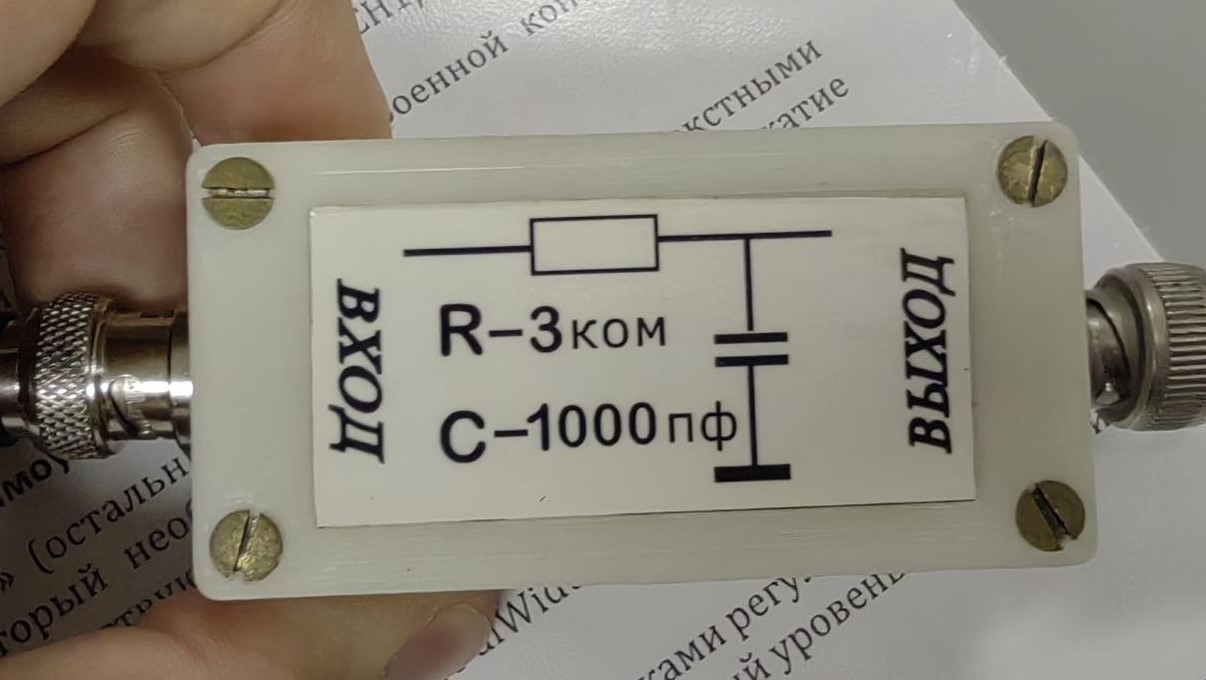
\includegraphics[width=0.8\linewidth]{f20.jpg}}
            \caption{$RC$-фильтр низких частот.}
            \label{f20}
        \end{minipage}
        \begin{minipage}[h]{0.5\linewidth}
            \center{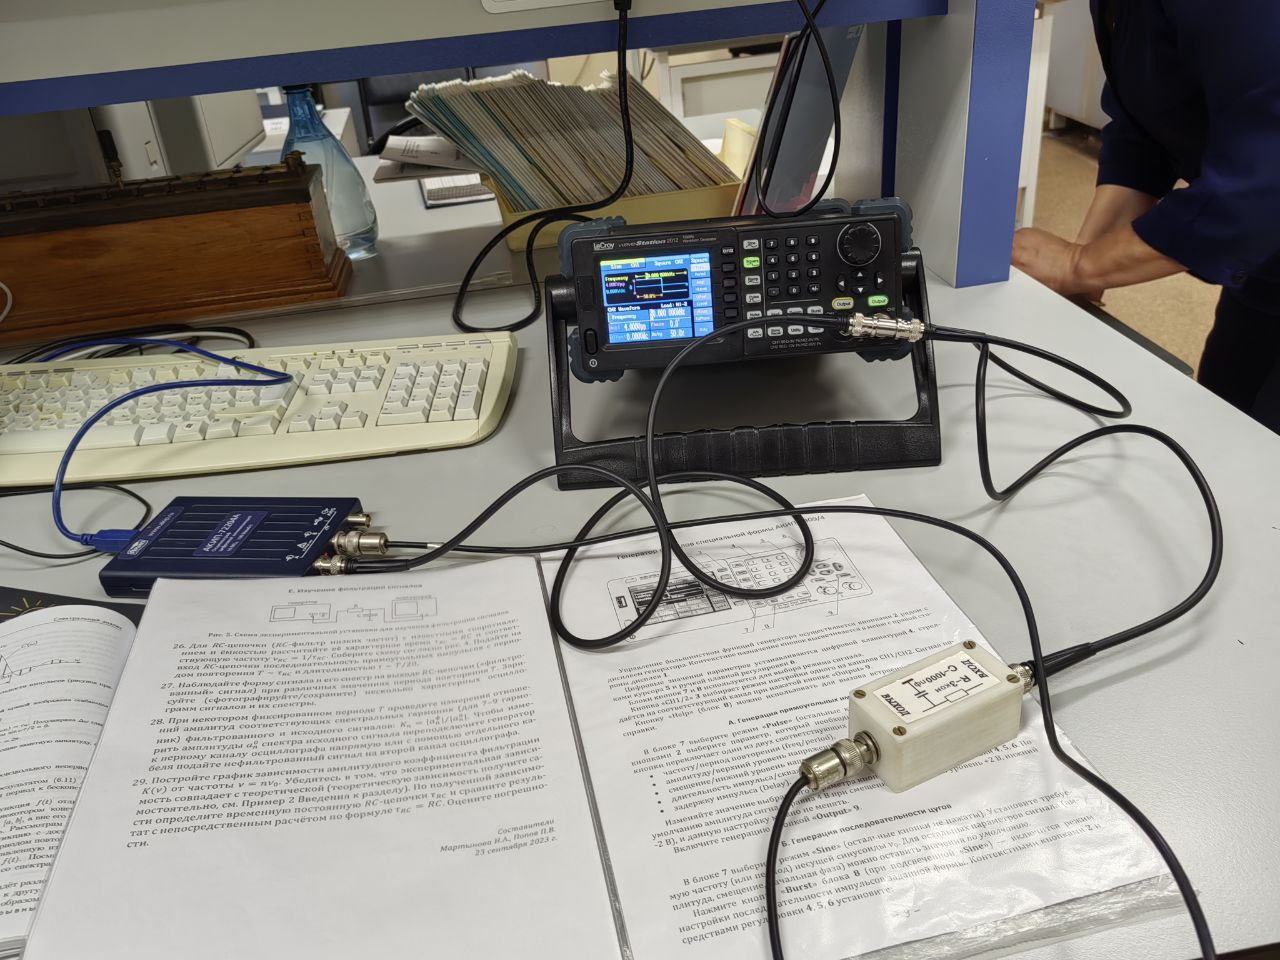
\includegraphics[width=0.8\linewidth]{f21.jpg}}
            \caption{Собранная схема.}
            \label{f21}
        \end{minipage}
        \begin{minipage}[h]{0.5\linewidth}
            \center{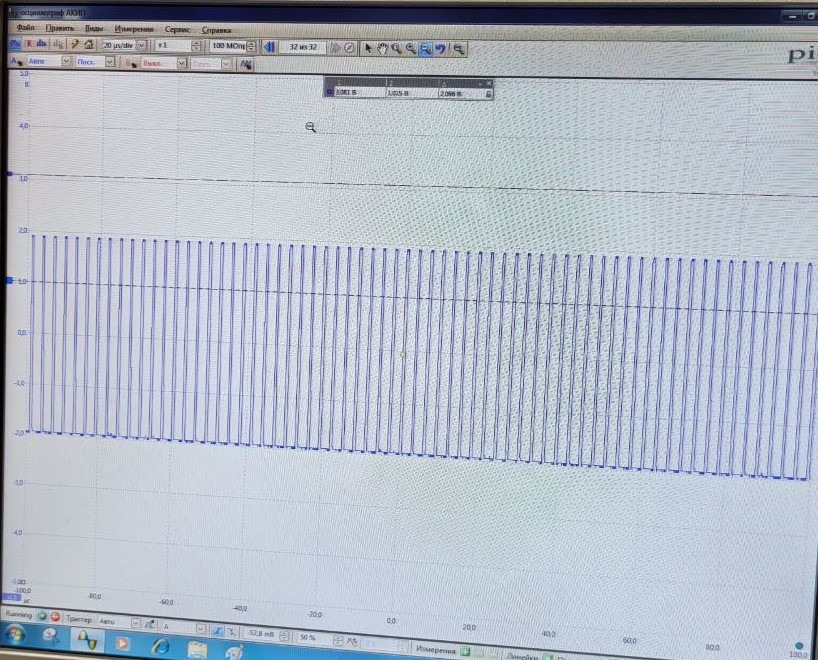
\includegraphics[width=0.8\linewidth]{f22.jpg}}
            \caption{Форма сигнала.}
            \label{f22}
        \end{minipage}
        \begin{minipage}[h]{0.5\linewidth}
            \center{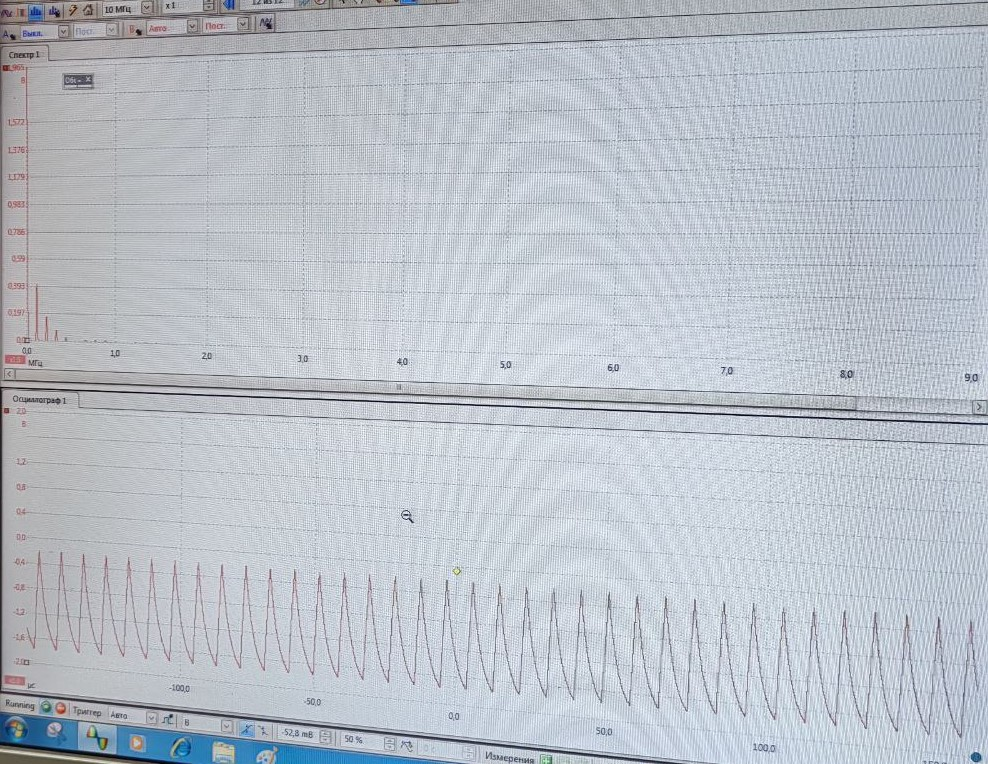
\includegraphics[width=0.8\linewidth]{f23.jpg}}
            \caption{Наблюдаемая форма сигнала и его спектр (1).}
            \label{f23}
        \end{minipage}
        \begin{minipage}[h]{0.5\linewidth}
            \center{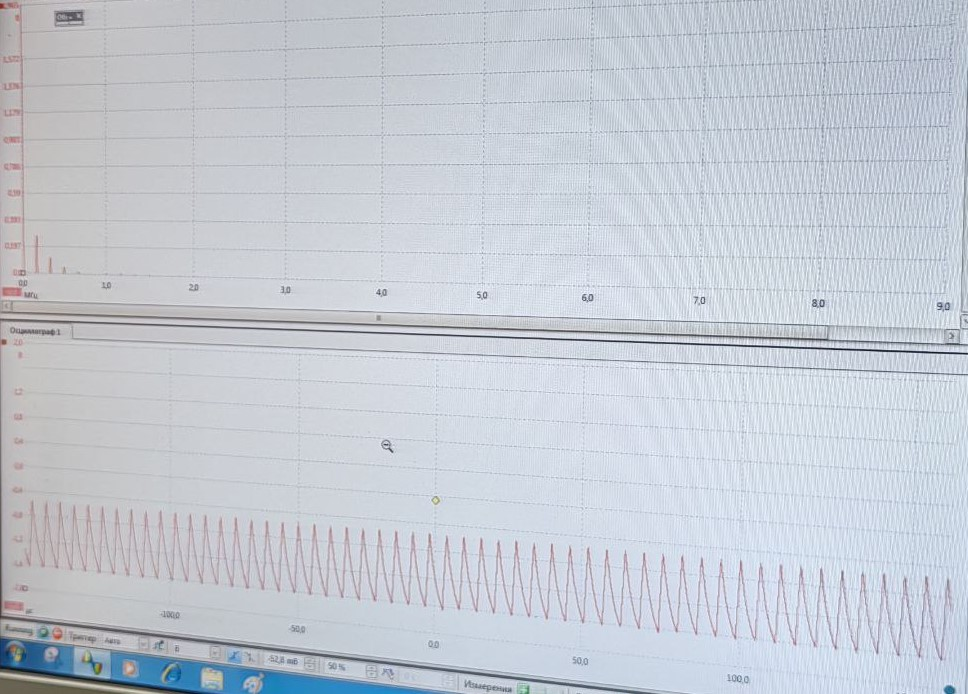
\includegraphics[width=0.8\linewidth]{f24.jpg}}
            \caption{Наблюдаемая форма сигнала и его спектр (2).}
            \label{f24}
        \end{minipage}
        \begin{minipage}[h]{0.5\linewidth}
            \center{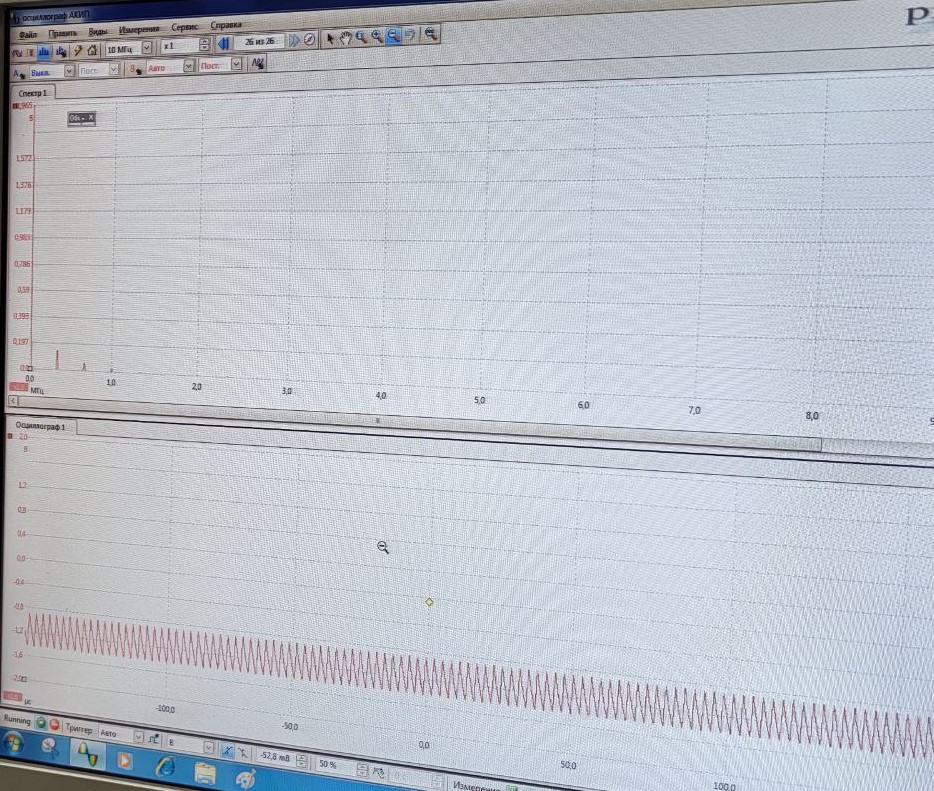
\includegraphics[width=0.8\linewidth]{f25.jpg}}
            \caption{Наблюдаемая форма сигнала и его спектр (3).}
            \label{f25}
        \end{minipage}
    \end{figure}

    \item Наблюдаем форму сигнала и его спектр при выходе $RC$-цепочки ("фильтрованный" сигнал) при различных значениях периода повторения $T$. Несклько случаев приведены на картинках \ref{f23}, \ref{f24}, \ref{f25}.

    \item При некотором фиксированном периоде $T = 6 \text{мкс}$ проведём измерения отношений амплитуд соответствующих спектральных гармоник фидбтрованного и исходного сигналов: $K_{n} = |a_{n}^{ф}|/|a_{n}^{0}|$. Чтобы измерить амплитуды $a_{n}^{0}$ спектра исходного сигнала, с помощью отдельного кабеля подадим екфильтрованный согнал на второй канал осциллографа. Результаты занесём в таблицу \ref{tab7}.


    \begin{table}[h]
	\centering
		\begin{tabular}{|c|c|c|c|}
			\hline
                $n$ & $|a_{n}^{ф}|, \text{ус.ед.}$ & $|a_{n}^{0}|, \text{ус.ед.}$ & $K_{n}$ \\ \hline
                1 & 0.711 & 1.015 & 0.7 \\ \hline
                2 & 0.294 & 0.822 & 0.16 \\ \hline
                3 & 0.132 & 0.546 & 0.24 \\ \hline
                4 & 47.23 & 254.2 & 0.19 \\ \hline
                5 & 29.56 & 166.3 & 0.18 \\ \hline
		\end{tabular}
            \hspace{.02\textwidth}
            \begin{tabular}{|c|c|c|c|}
			\hline
                $n$ & $|a_{n}^{ф}|, \text{ус.ед.}$ & $|a_{n}^{0}|, \text{ус.ед.}$ & $K_{n}$ \\ \hline
                6 & 25.27 & 233.8 & 0.11 \\ \hline
                7 & 17.43 & 204.0 & 0.09 \\ \hline
                8 & 9.58 & 114.6 & 0.08 \\ \hline
                9 & 8.016 & 91.84 & 0.087 \\ \hline
		\end{tabular}
	\caption{Результаты измерений}
        \label{tab7}
    \end{table}

    Проверим, что экспериментальная зависимость совпадает с теоретической $K = \frac{1}{\tau_\text{RC}} \int_0^t f(t')dt'$. Т.к. мы подаём последовательность прямоугольных импульсов, то правая часть зависит линейно от $t$, т.е. обратно пропорционально $\nu$. График соответствует этой зависимости.
    
\end{enumerate}

\subsection{Выводы}

В этой работе мы изучили спектральный состав периодических электрических сигналов, а именно:

\begin{enumerate}
    \item исследовали спектр периодической последовательности прямоугольных импульсов, проверили соотношения неопределённости;
    \item наблюдпли спектр периодической последовательности цугов;
    \item изучили фильтрацию сигналов.
\end{enumerate}


    \begin{figure}[h]
        \centering
        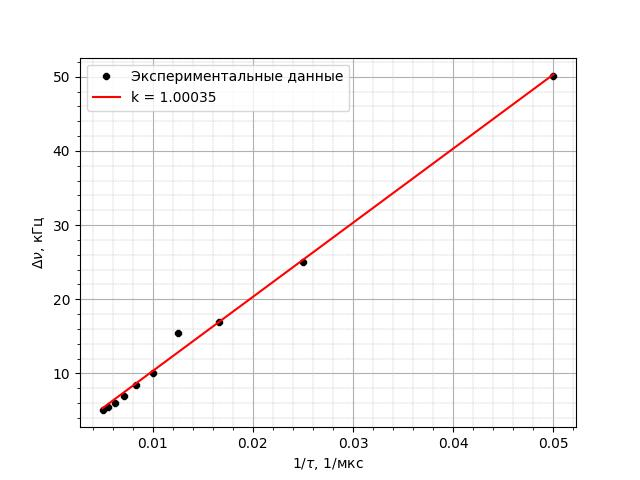
\includegraphics[width=14cm]{image1.jpg}
        \caption{Графическая зависимость ширины спектра сигнала от длительности импульса}
        \label{graf1}
    \end{figure}
    \begin{figure}[h]
        \centering
        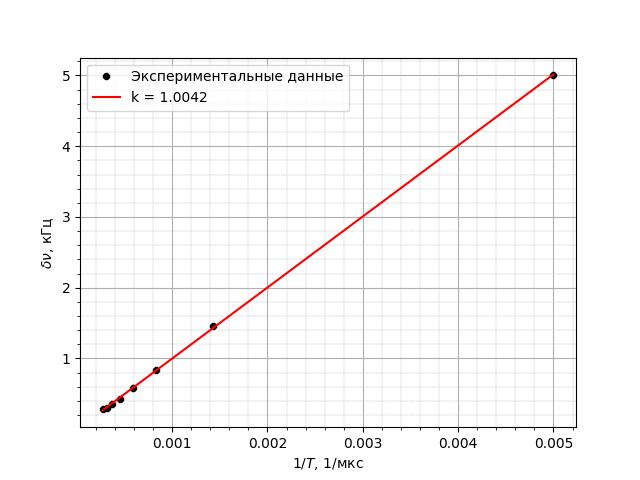
\includegraphics[width=14cm]{image2.jpg}
        \caption{Графическая зависимость разности частот между соседними гармониками от периода повторений}
        \label{graf2}
    \end{figure}
    \begin{figure}[h]
        \centering
        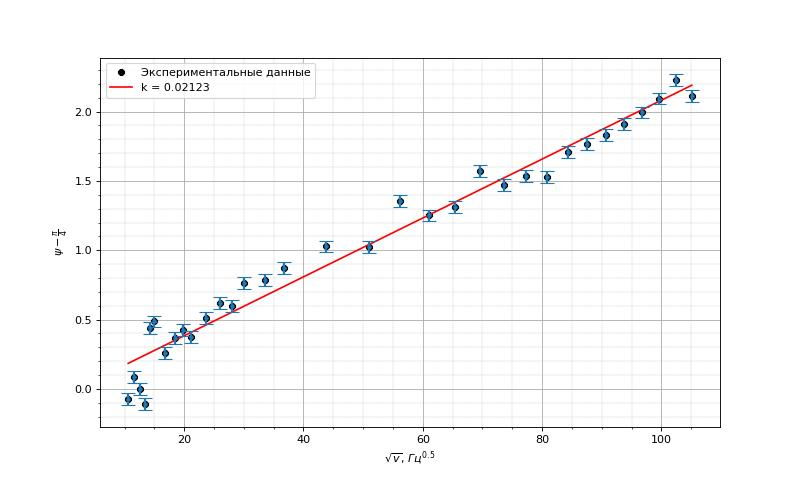
\includegraphics[width=14cm]{image3.jpg}
        \caption{Графическая зависимость отношения боковой частоты к основной от глубины модуляции}
        \label{graf3}
    \end{figure}
    \begin{figure}[h]
        \centering
        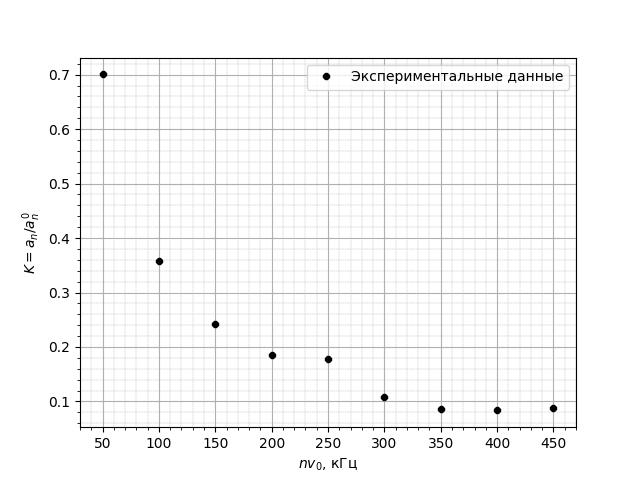
\includegraphics[width=14cm]{image4.jpg}
        \caption{Графическая зависимость $K(\nu)$}
        \label{graf3}
    \end{figure}


\end{document}
